\artigotrue
\chapter{Do more detailed environmental covariates deliver more accurate soil maps?}
\label{chap:chap05}

% User defined commands
\def\elev{\texttt{ELEV}} % elevation
\def\slp{\texttt{SLP}}   % slope
\def\asp{\texttt{ASP}}   % aspect
\def\nor{\texttt{NOR}}   % northernness
\def\acc{\texttt{ACC}}   % flow accumulation
\def\twi{\texttt{TWI}}   % topographic wetness index
\def\spi{\texttt{SPI}}   % stream power index
\def\tpi{\texttt{TPI}}   % topographic position index
\def\ndvi{\texttt{NDVI}} %
\def\savi{\texttt{SAVI}} %
\def\sibcs{Brazilian System of Soil Classification}

\def\englishkeys{Digital Soil Mapping, Linear Mixed Model, Auxiliary 
  Information, Variable Selection, Model Accuracy, Soil Mapping Cost}
  
\begin{chapterabstract}{english}{\englishkeys}
In this study we evaluated whether investing in more spatially detailed 
environmental covariates improves the accuracy of digital soil maps. We used a 
case study from Southern Brazil to map clay content (CLAY), organic carbon 
content (SOC), and effective cation exchange capacity (ECEC) of the topsoil for
a $\sim$~2,000~ha area located on the edge of the plateau of the Paraná 
Sedimentary Basin. Five covariates, each with two levels of spatial detail were
used: area-class soil maps, digital elevation models (DEM), geologic maps, land
use maps, and satellite images. Thirty-two multiple linear regression models 
were calibrated for each soil property using all spatial detail combinations of
the covariates. For each combination, stepwise regression was used to select 
predictor variables incorporated in the model. Model evaluation was done using 
the adjusted R-square of the regression. The baseline model, calibrated with the
less detailed version of each covariate, and the best performing model were used
to calibrate two linear mixed models for each soil property. Model parameters 
were estimated using restricted maximum likelihood. Spatial prediction was 
performed using the empirical best linear unbiased predictor. Validation of 
baseline and best performing linear multiple regression and linear mixed models
was done using cross-validation. Results show that for CLAY the prediction 
accuracy did not considerably improve by using more detailed covariates. The 
amount of variance explained increased only $\sim$~2 percentage points (pp), 
less than that obtained by including the kriging step, which explained 4~pp. On
the other hand, prediction of SOC and ECEC improved by $\sim$~13~pp when the 
baseline model was replaced by the best performing model. Overall, the increase
in prediction performance was modest and may not outweigh the extra costs of 
using more detailed covariates. It may be more efficient to spend extra 
resources on collecting more soil observations, or increasing the detail of only
those covariates that have the strongest improvement effect. In our case study,
the latter would only work for SOC and ECEC, by investing in a more detailed 
land use map and possibly also a more detailed geologic map and DEM.
\end{chapterabstract}

\def\portuguesekeys{Mapeamento Digital do Solo, Modelo Linear Misto, Informação 
Auxiliar, Seleção de Variáveis, Acurácia do Modelo, Custo do Mapeamento do Solo}
\begin{chapterabstract}{brazilian}{\portuguesekeys}
Neste estudo nós avaliamos se investir em covariáveis ambientais espacialmente
mais detalhadas aumenta a acurácia dos mapas digitais do solo. Nós usamos um 
estudo de caso no sul do Brasil para mapear o conteúdo de argila (CLAY), o
conteúdo de carbono orgânico (SOC), e capacidade de troca de cátions efetiva 
(ECEC) da camada superficial do solo de uma área de $\sim$~2000~ha localizada
na borda do planalto da Bacia Sedimentar do Paraná. Cinco covariáveis, cada uma
com dois níveis de detalhe espacial, foram usadas: mapa areal-categórico de solo,
modelos digitais de elevação (DEM), mapas geológicos, mapas de uso da terra, e 
imagens de satélite. Trinta e dois modelos de regressão linear múltipla foram
calibrados para cada propriedade do solo usando todas as combinações de detalhe
espacial das covariáveis. Para cada combinação, stepwise regression foi usada 
para selecionar as variáveis preditoras incorporadas no modelo. A avaliação dos
modelos foi feita usando o R-quadrado ajustado da regressão. O modelo baseline, 
calibrado com a versão menos detalhada de cada covariável, e o modelo com o 
melhor desempenho, foram usados para calibrar dois modelos lineares mistos para
cada propriedade do solo. Parâmetros dos modelos foram estimados usando 
restricted maximum likelihood. Predições espaciais foram realizadas usando o 
empirical best linear unbiased predictor. Validação-cruzada foi usada para 
validar os modelos de regressão linear múltipla e dos modelos lineares mistos 
de linha de base e com melhor desempenho. Os resultados mostram que para CLAY a 
acurácia da predição não aumentou consideravelmente por usar covariáveis mais
detalhadas. A quantidade de variância explicada aumentos apenas $\sim$~2 pontos
percentuais (pp), menos do que obtido pela inclusão do passo de krigagem, que
explicou 4-pp. Por outro lado, a predição de SOC e ECEC aumentos em $\sim$~13~pp
quando o modelo de base foi substituído pelo modelo com melhor desempenho. Em 
geral, o aumento no desempenho preditivo foi modesto e pode não sobrepor os 
custos adicionais do uso de covariáveis mais detalhadas. Pode ser mais eficiente
investir recursos adicionais na coleta de mais observações do solo, ou no 
aumento do detalhe apenas da covariável que tem o efeito de aumento mais forte.
Em nosso estudo, a última funcionaria apenas para SOC e ECEC pelo investimento
em um mapa de uso da terra mais detalhado e, possivelmente, também em um mapa 
geológico e DEM mais detalhados.
\end{chapterabstract}

\formatchapter

\section{Introduction}
\label{sec:intro}

Digital soil mapping relies on the use of statistical models to produce digital representations of spatial soil 
distribution using point soil observations and spatially exhaustive environmental covariates 
\cite{McBratneyEtAl2003, ScullEtAl2003, Florinsky2012}. Three important weaknesses in the statistical 
soil distribution modelling approach can be pointed out. First, it requires sufficient and appropriately 
distributed point soil data within the area being mapped \cite{CarreEtAl2007a}. Second, the model structure 
explores only the empirical relationship among environmental conditions and soil properties, being
less comprehensive than soil-landscape process models \cite{Grunwald2009}. Last, the covariates are only 
approximations of the true environmental conditions that helped shape the soil. They serve only as proxies 
(surrogates) of the current environmental conditions, which in many cases are different from the past 
conditions under which pedogenesis took place \cite{HeuvelinkEtAl2001}. In spite of these weaknesses, digital 
soil mapping has proven very successful in the past decades in producing soil property maps that capture the 
main patterns of soil spatial variation \cite{MooreEtAl1993, McBratneyEtAl2000, Grunwald2009}.

More recently, there has been a growing interest in understanding how the characteristics of the environmental 
covariates influence the success of digital soil mapping -- this study contributes to this effort. It is 
commonly accepted that the more resources are spent on the construction of a covariate and the more spatial 
information it has, the more accurately it describes the environmental conditions \cite{HupyEtAl2004, 
HenglEtAl2013a}. It is also generally believed that such \textit{more detailed} covariates will be more 
valuable for digital soil mapping and lead to more accurate soil property predictions \cite{CavazziEtAl2013, 
MaynardEtAl2014}. If these more detailed covariates convey more information and represent more adequately the 
environmental conditions -- the drivers of soil forming processes --, then it is fair to expect that they 
improve the accuracy of the resulting soil maps. However, some studies have shown the contrary 
\cite{ThompsonEtAl2001, EldeiryEtAl2008, KimEtAl2014}. For example, the window size at which DEM derivatives 
are calculated can be more important than the spatial resolution of the DEM \cite{Wood1996, ZhuEtAl2008, 
BehrensEtAl2010a}. The uncertainty about the added value of using more detailed covariates is of concern for 
those seeking to use resources efficiently, because using more detailed covariates generally increases soil 
mapping costs \cite{ShiEtAl2012}.

The objective of this study was to evaluate whether investing in more detailed environmental covariates 
improves the accuracy of digital soil maps. The main difference of our study to previous ones is that we use a 
rigorous statistical approach to assess the added value of using five more detailed covariates simultaneously. 
We used a case study in Brazil to compare the accuracy of digital maps of the clay content, organic carbon 
content and effective cation exchange capacity of the topsoil as obtained from regression kriging on the five 
covariates, whereby each covariate was evaluated on two levels of spatial detail.

\section{Material and Methods}
\label{sec:methods}

\subsection{Study area and soil data}
\label{subsec:soil-data}

The study area constitutes a small catchment ($\sim$~2,000~ha) located on the southern edge of the plateau of 
the Paraná Sedimentary Basin, Rio Grande do Sul, Brazil (\autoref{fig:location}). The climate is classified as 
Cfa (K\"oppen -- subtropical humid without a dry season) with mean annual temperature of 19.3$^{\circ}$C, and 
mean annual precipitation of 1,708~mm, well distributed throughout the year \cite{Maluf2000}. Relief varies 
between plain (slope between 0 and 3\%) and mountainous (slope between 45 and 100\%), and elevations range 
between 140 and 475~m. Geology consists of basic, intermediate and acid igneous rocks (rhyolite-rhyodacite and 
andesite-basalt) of the Cretaceous period, consolidated sedimentary rocks (aeolian and fluvial sandstones) of 
the Triassic and Jurassic periods, and non-consolidated (fluvial and colluvial deposits) of the Quaternary 
period \cite{GasparettoEtAl1988, MacielFilho1990, Sartori2009}. Native semi-deciduous forests occupy more than 
half of the area, followed by native grassland used for animal husbandry, semi-deciduous shrubland, annual 
crop agriculture, forestry (Eucalyptus), urban areas, and artificial water bodies \cite{SamuelRosaEtAl2011a}.

 \begin{figure}[!ht]
    \centering
    \begin{minipage}[b]{95mm}
      \subcaption{}
      \label{fig:brazil}
      \centering
      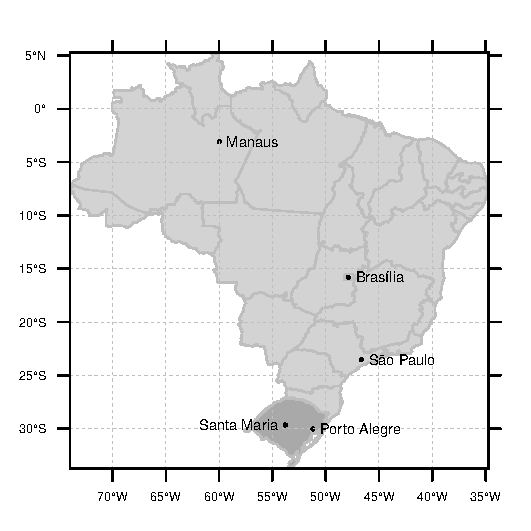
\includegraphics[width=90mm]{chap01FIG1a}
    \end{minipage}
    \begin{minipage}[b]{95mm}
      \subcaption{}
      \label{fig:points}
      \centering
      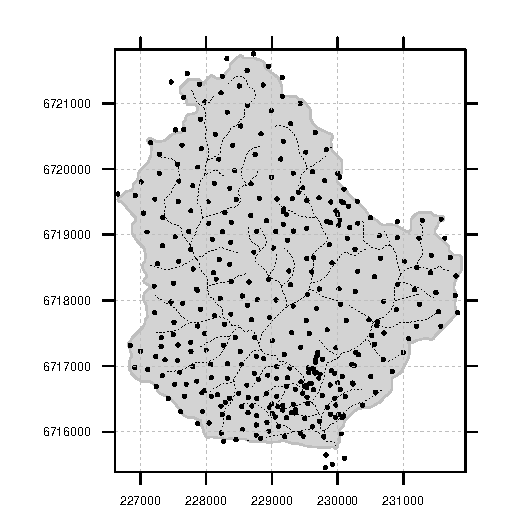
\includegraphics[width=90mm]{chap01FIG1b}
    \end{minipage}
  \caption{Location of the study area in Santa Maria (a) and spatial 
  distribution of the point soil observations and drainage network (b).}
  \label{fig:location}
 \end{figure}

A dataset containing $n=350$ point soil observations collected between 2004 and 2011 \cite{PedronEtAl2006b, 
SamuelRosaEtAl2011a, MiguelEtAl2012, Samuel-RosaEtAl2013} was used in this study (available at 
\url{https://github.com/samuel-rosa/dnos-sm-rs}). Sampling locations were selected purposively and by 
convenience \cite{Samuel-RosaEtAl2014b}. Three soil pits were opened within an area of about 100~m$^2$ at most 
sampling locations to obtain composite samples of the topsoil for laboratory analysis. Soil was collected to a 
depth of 20~cm or less when soil depth was smaller than 20~cm. A few observations ($n = 10$) correspond to 
individual samples collected up to 30~cm. Sampling depth ranges from 2 to 30~cm, with a mean of 17.3~cm. We 
assumed that the vertical, horizontal and temporal support differences between soil samples is negligible for 
the purpose of this study.

Three soil properties (fine earth fraction, $<2$~mm) were explored: clay content 
(CLAY,~\si{\gram\per\kilo\gram}), organic carbon content (SOC,~\si{\gram\per\kilo\gram}), and effective cation 
exchange capacity (ECEC,~mmol~kg$^{-1}$). CLAY was determined by the pipette method. SOC was determined using 
wet digestion. ECEC was calculated as the sum of exchangeable bases plus exchangeable acidity. The soil 
properties selected were expected to present different patterns of spatial variation and correlation with the 
most dominant factors of soil formation \cite{Jenny1941} in the area: organisms (\textit{O}), relief 
(\textit{R}), and parent material (\textit{P}). CLAY was presumed to have a stronger relation with \textit{P}, 
while SOC was expected to be more correlated with \textit{O}. Because the soils of the study area were strongly 
eroded due to intense agriculture in the 20th century, both CLAY and SOC were also expected to be closely 
related with \textit{R}. Finally, ECEC was expected to be strongly correlated with \textit{P} and \textit{O}, 
which is supported by its natural relationship with both CLAY and SOC.

 \begin{figure}[!ht]
   \centering
    \begin{minipage}[b]{63mm}
      \subcaption{}
      \centering
      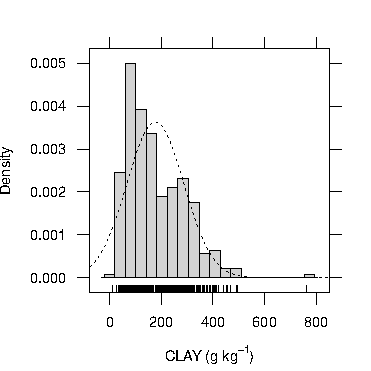
\includegraphics[width=63mm]{chap01FIG2a}
    \end{minipage}
    \begin{minipage}[b]{63mm}
      \subcaption{}
      \centering
      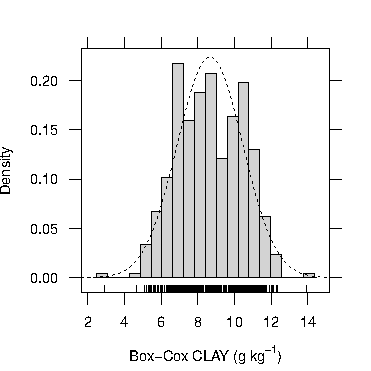
\includegraphics[width=63mm]{chap01FIG2d}
    \end{minipage}
    \begin{minipage}[b]{63mm}
      \subcaption{}
      \centering
      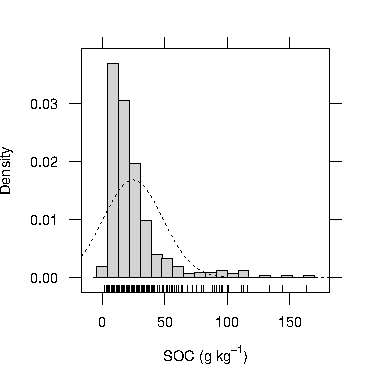
\includegraphics[width=63mm]{chap01FIG2b}
    \end{minipage}
    \begin{minipage}[b]{63mm}
      \subcaption{}
      \centering
      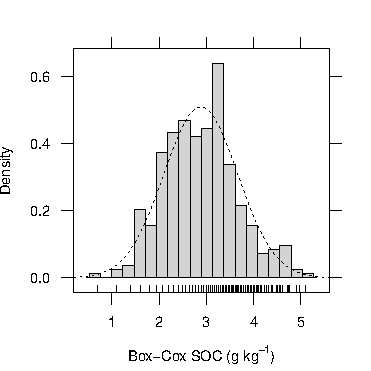
\includegraphics[width=63mm]{chap01FIG2e}
    \end{minipage}
    \begin{minipage}[b]{63mm}
      \subcaption{}
      \centering
      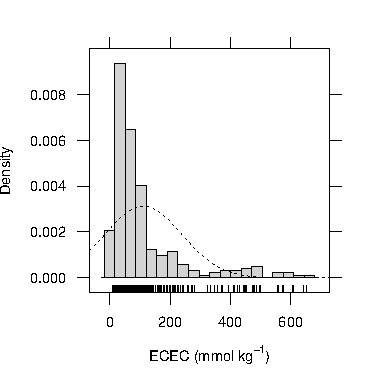
\includegraphics[width=63mm]{chap01FIG2c}
    \end{minipage}
    \begin{minipage}[b]{63mm}
      \subcaption{}
      \centering
      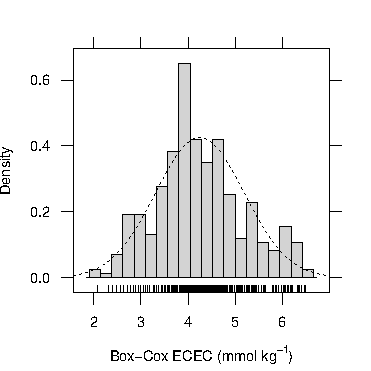
\includegraphics[width=63mm]{chap01FIG2f}
    \end{minipage}
  \caption{Histogram, empirical density function, and summary statistics of CLAY (a, b), SOC (c, d), and ECEC 
(e, f) in the original (left) and Box-Cox feature spaces (right).}
  \label{fig:soil-properties}
 \end{figure}

Point soil data, here denoted by $Z(s)$, showed a positive skew (\autoref{fig:soil-properties}) and was 
normalized, $Z'(s)$, using the Box-Cox family of power transformations, where $Z'(s) = (Z(s)^{\lambda} - 1) / 
\lambda$, if $\lambda > 0$, and $Z'(s) = log(Z(s))$, if $\lambda = 0$ \cite{DiggleEtAl2007}. Lambda ($\lambda$) 
values were selected empirically \cite{FoxEtAl2011}. Because the resulting distribution of the back-transform 
(see \autoref{subsec:validation}) has no expectation when $\lambda<0$ \cite{RibeiroEtAl2001}, a logarithm 
transformation ($\lambda=0$) was used when a negative $\lambda$ was estimated (SOC and ECEC).

\subsection{Environmental covariates}
\label{subsec:sources}

Five freely available environmental covariates were evaluated in this study, each with two levels of spatial 
detail: area-class soil maps (\texttt{soil}), geologic maps (\texttt{geo}), land use maps (\texttt{land}), 
digital elevation models (\texttt{dem}), and satellite images (\texttt{sat}). Each pair was composed by 
covariates that were produced separately from scratch using different data sources and/or production methods, 
thus demanding different amounts of resources (time, workforce, budget, technology, etc.). In this study,
the level of spatial detail of an environmental covariate is a function of the components of its production 
process such as the cartographic ratio (\texttt{soil}, \texttt{geo} and \texttt{land}), spatial sampling 
support (\texttt{sat}), number and diversity of data sources explored (\texttt{dem}), and quantity of spatial 
data used (all five). Thus, the reader should bear in mind that our definition of spatial detail is broader 
than spatial resolution or spatial scale. It should also not be confounded with spatial support 
\cite{WebsterEtAl2007} or thematic detail \cite{Rossiter2000}.

The environmental covariates were transformed to predictor variables that were used in the geostatistical 
modelling. Since the transformation is different for categorical and continuous covariates, the procedures are 
explained below for each type separately.

\subsubsection*{Categorical predictor variables}
\label{subsubsec:categorical-covars}

Area-class soil maps, geologic maps and land use maps are categorical environmental covariates (factors). 
Mapping units are the $k$ factor levels that are transformed to as many dummy (indicator, binary) variables as 
there are factor levels, before model calibration. Each dummy variable receives a value equal to one (1) when a 
given class is present, and zero (0) otherwise \cite{Everitt2006}. If the number of point soil observations 
falling inside the spatial domain of a mapping unit is too small to accurately estimate a regression 
coefficient (we used a threshold of $n=15$ observations), the mapping unit is merged with a similar mapping 
unit prior to calculating dummy variables. The resulting generalized categorical covariate maps are shown in 
\autoref{fig:cat-covars}. The binary maps are the categorical predictor variables.

\noindent\textit{Soil maps}. The less detailed soil map (\soilOld) was published with a \scale{100,000} and has 
five mapping units \cite{AzolinEtAl1988} (\autoref{fig:soil-old}). It was produced using existing soil maps and 
technical reports (\scale{750,000}) \cite{Brasil1973}, aerial photographs (\scale{60000}), topographic maps 
(\scale{50,000}), and sparse point soil observations along the road network. The more detailed soil map 
(\soilNew) was prepared with a \scale{25000} and has eight mapping units \cite{MiguelEtAl2012}
(\autoref{fig:soil-new}). It was produced using high spatial resolution satellite images (65~cm), existing soil 
maps and technical reports published with a \scale{50,000} \cite{Poelking2007} and 1:25,000 
\cite{PedronEtAl2006b}, topographic maps (\scale{25,000}), and descriptions from $\sim$~350 point soil 
observations. Five dummy predictor variables were derived from \soilOld{} and seven from \soilNew{} 
(\autoref{tab:soil-covars}).

 \begin{figure}[!ht]
    \centering
    \begin{minipage}[b]{63mm}
       \subcaption{Cartographic scale: 1:100,000}
       \label{fig:soil-old}
       \centering
       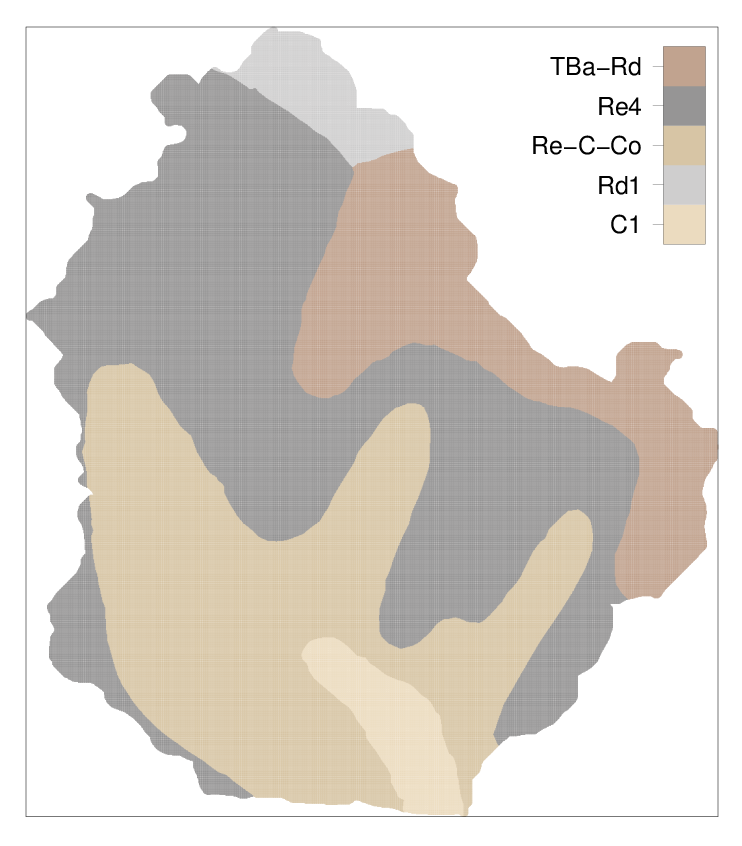
\includegraphics[width=60mm]{chap01FIG3a}
    \end{minipage}
    \begin{minipage}[b]{63mm}
       \subcaption{Cartographic scale: 1:25,000}
       \label{fig:soil-new}
       \centering
       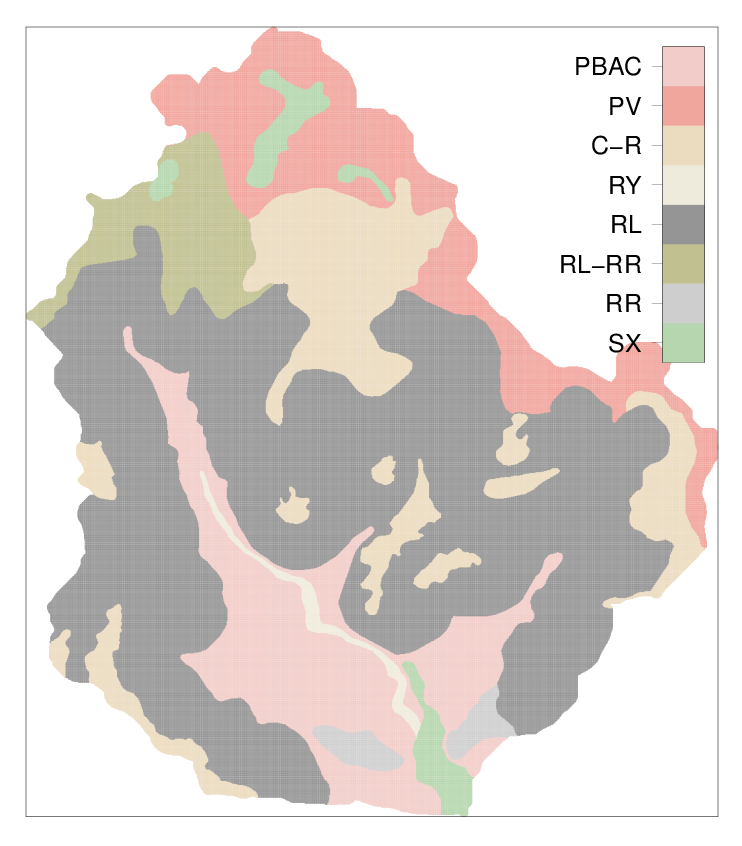
\includegraphics[width=60mm]{chap01FIG3d}
    \end{minipage}    
    \begin{minipage}[b]{63mm}
       \subcaption{Cartographic scale: 1:50,000}
       \label{fig:geo-old}
       \centering
       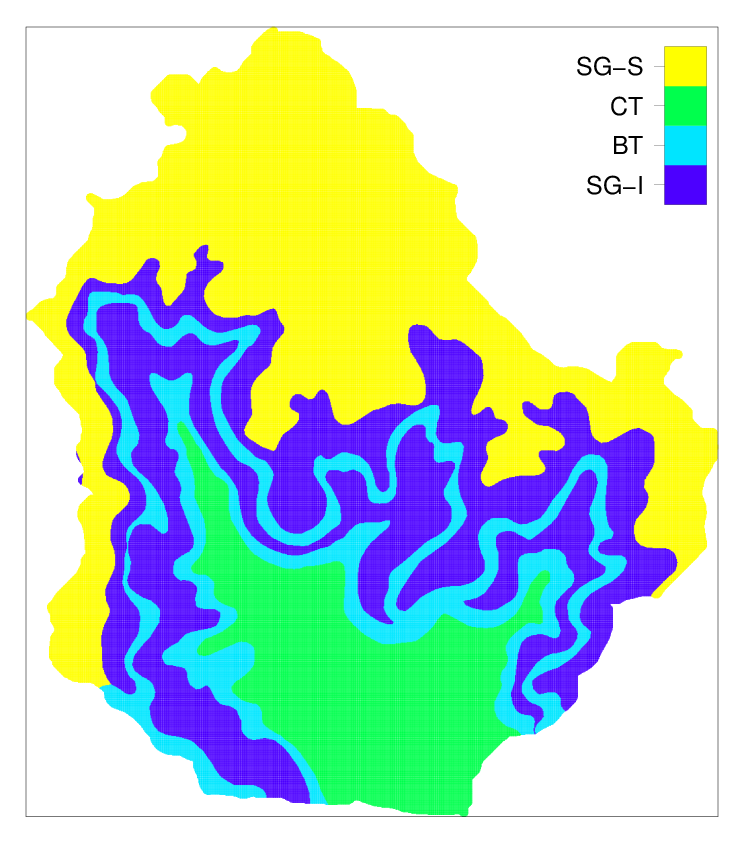
\includegraphics[width=60mm]{chap01FIG3b}
    \end{minipage}
    \begin{minipage}[b]{63mm}
       \subcaption{Cartographic scale: 1:25,000}
       \label{fig:geo-new}
       \centering
       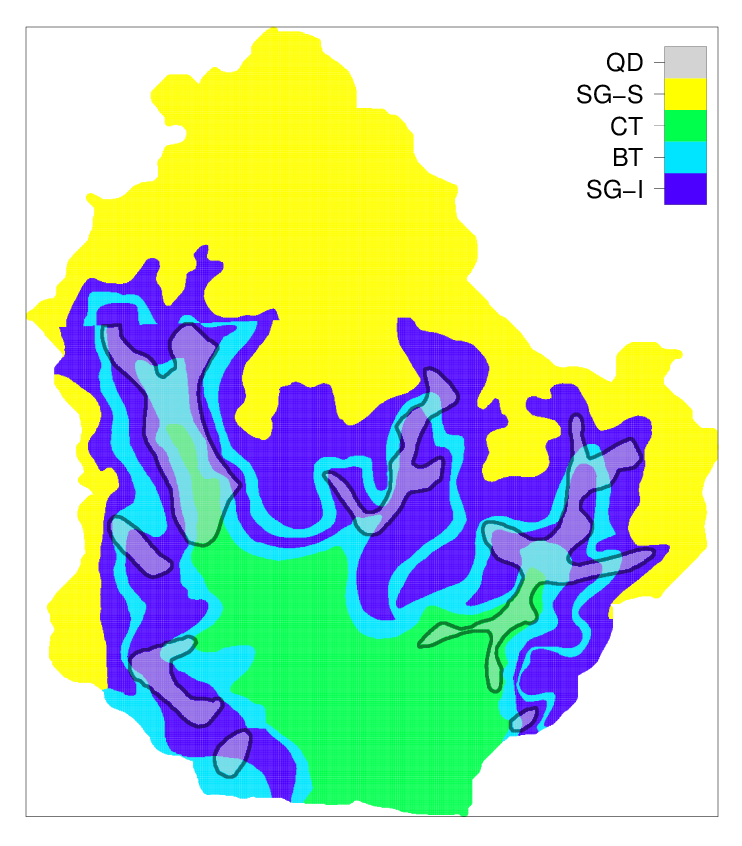
\includegraphics[width=60mm]{chap01FIG3e}
    \end{minipage}
    \begin{minipage}[b]{63mm}
       \subcaption{Cartographic scale: 1:500,000}
       \label{fig:land-old}
       \centering
       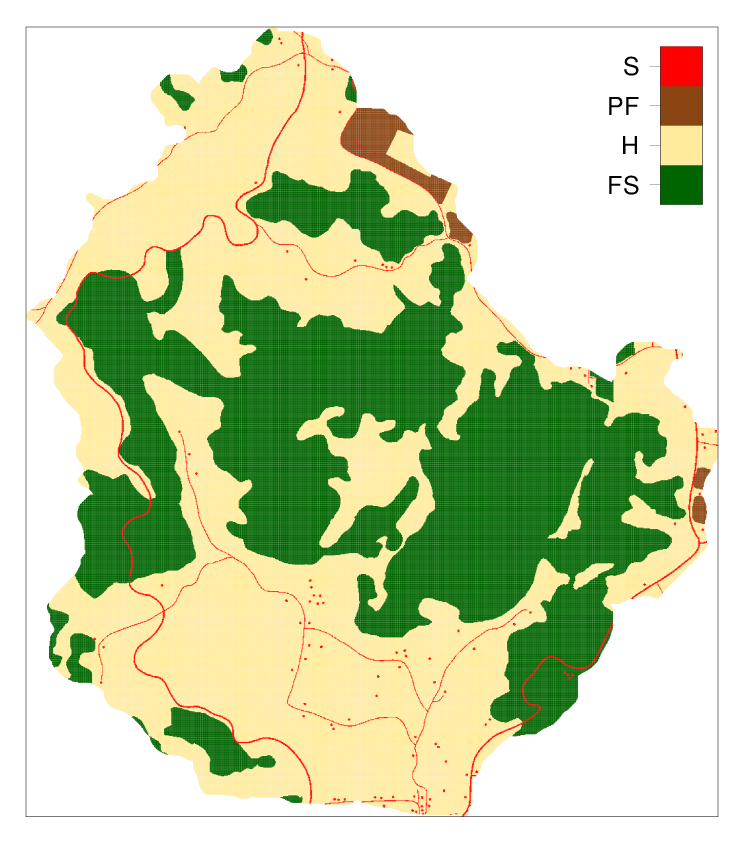
\includegraphics[width=60mm]{chap01FIG3c}
    \end{minipage}
    \begin{minipage}[b]{63mm}
       \subcaption{Cartographic scale: 1:2,000}
       \label{fig:land-new}
       \centering
       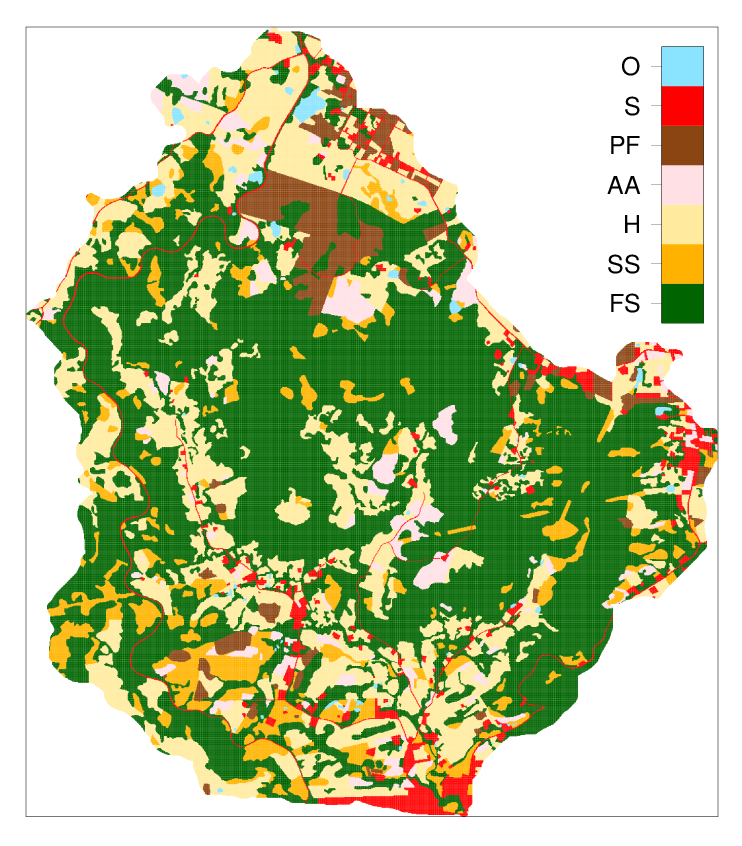
\includegraphics[width=60mm]{chap01FIG3f}
    \end{minipage}
   \caption{Area-class soil maps (a, b), geologic maps (c, d), and land use 
   maps (e, f) compared in our study. The less detailed version is displayed 
   at the left, while the more detailed version is shown on the right. Legend 
   abbreviations and derived dummy variables are described in Tables 
   \ref{tab:soil-covars}--\ref{tab:land-covars}.}
  \label{fig:cat-covars}
\end{figure}

\noindent\textit{Geologic maps}. The less detailed geologic map (\geoOld) was produced using topographic maps 
with \scale{50,000} \cite{GasparettoEtAl1988} (\autoref{fig:geo-old}). The more detailed geologic map (\geoNew) 
was produced using topographic maps with \scale{25,000}, and includes the location of overlaying Quaternary 
sedimentary deposits \cite{MacielFilho1990} (\autoref{fig:geo-new}). \geoNew{} did not cover a small part in 
the North of the study area, where \geoOld{} was used instead (this strategy was approved by experts on the 
local geology). The mapping unit of both geologic maps depicting the Caturrita Formation was used indirectly 
by deriving dummy predictor variables from all other individual mapping units. Three dummy predictor variables 
were derived from \geoOld{} and four from \geoNew{} (\autoref{tab:geology-covars}).

\noindent\textit{Land use maps}. The less detailed land use map (\landOld) was produced by manually digitizing 
land use data included in topographic maps with a \scale{25000} \cite{DSG1980, DSG1992, DSG1992a} 
(\autoref{fig:land-old}). The more detailed land use map (\landNew) was prepared (\scale{2,000}) by manual 
digitization using 65~cm spatial resolution satellite images covering the years 2008 and 2009 
\cite{SamuelRosaEtAl2011a} (\autoref{fig:land-new}). Mapping units depicting human settlements and water bodies 
($n=0$) were not masked out from the prediction grid and were merged with other mapping units to derive dummy 
predictor variables. Five dummy predictor variables were derived from \landNew{} and two from \landOld{} 
(\autoref{tab:land-covars}).

\subsubsection*{Continuous predictor variables}
\label{subsubsec:continuous-covars}

The less detailed DEM (\demOld) is the hole-filled SRTM DEM version~4 \cite{JarvisEtAl2008} 
(\autoref{fig:dem-old}). The spatial sampling support of the SRTM DEM is 1~arc-second ($\sim$~30~m), but 
elevation data were aggregated to 3~arc-seconds ($\sim$~90~m) for public release in regions outside the United 
States \cite{ReuterEtAl2007}. The more detailed DEM (\demNew) was produced by interpolating contour lines with 
vertical spacing of 10~m along with data about the drainage network, lakes and peaks digitized from topographic 
maps with \scale{25,000} (\autoref{fig:dem-new}). Interpolation to 5-m pixel size was performed using a 
hydrologically correct algorithm implemented in 
\href{http://resources.arcgis.com/en/help/main/10.1/index.html#/How_Topo_to_Raster_works/009z0000007m000000/}{ 
ArcGIS\textregistered{}} software by ESRI \cite{Hutchinson1989}. Contour line artefacts were minimized using a 
seven by seven low-pass filter (\grass{r.neighbors}). The window size was chosen such that the smoothed DEM 
best matched the original contour map while also respecting the original drainage network pattern.

\ctable[
   caption  = {Description of the $p=12$ dummy predictor variables derived from the two soil maps.},
   label    = tab:soil-covars,
   notespar,
   pos      = !ht,
%    doinside = \scriptsize\setstretch{1.1},
   doinside = \scriptsize
   ]{l p{0.85\textwidth} l}{
   \tnote[a]{Soil classification according to the old Brazilian classification (only for \citet{AzolinEtAl1988}), the current Brazilian classification \citep{SantosEtAl2013a}, and the international classification \citep{IUSSWorkingGroupWRB2007}.}
   \tnote[b]{Minimum Legible Delineation calculated following \citet{Rossiter2000}.}
   }{                                                                                                                    \FL
   Code                & Mapping unit(s) included and Description\tmark[a,b]                                             \ML
   \multicolumn{2}{l}{Source: \citet{AzolinEtAl1988}. Cartographic scale: 1:100,000. Minimum Legible Delineation: 40~ha.} \NN
   \texttt{SOIL\_100b} & \textit{Re4}. Shallow soils with low to high base saturation covering mountainous terrain (Solo Litólico Eutrófico/Distrófico relevo montanhoso; Neossolo Litólico Distrófico/Eutrófico; Distric/Eutric Leptosol). \NN 
   \texttt{SOIL\_100c} & \textit{Re-C-Co}. Shallow soils with high base saturation located in strongly sloping terrain (Solo Litólico Eutrófico relevo forte ondulado; Neossolo Litólico Eutrófico; Eutric Leptosol), low weathered soils (Cambissolo Eutrófico; Cambissolo Háplico Eutrófico; Eutric Cambisol), and colluvial deposits. \NN
   \texttt{SOIL\_100d} & \textit{TBa-Rd}. Deep, well-structured, low base saturation soils (Terra Bruna Estruturada álica; Nitossolo; Nitisol), and shallow soils (Solo Litólico; Neossolo Litólico; Leptosol). \NN
   \texttt{SOIL\_100e} & \textit{Rd1} and \textit{Re4}. \textit{Rd1} is composed mainly by shallow soils with low to high base saturation (Solo Litólico Distrófico/Eutrófico; Neossolo Litólico Distrófico/Eutrófico; Distric/Eutric Leptosol) located in slopping terrain. This dummy predictor variable is composed by shallow soils in both sloping and mountainous terrain. \NN
   \texttt{SOIL\_100f} & \textit{TBa-Rd} and \textit{C1}. \textit{C1} is composed by low weathered soils developed in lower landscape positions, close to drainage channels (Cambissolo Eutrófico; Cambissolo Eutrófico; Eutric Cambisol). This dummy predictor variable includes the best soil mapping units for crop agriculture among those identified in the soil survey. \NN
   &                                                                                                                     \NN
   \multicolumn{2}{l}{Source: \citet{MiguelEtAl2012}. Cartographic scale: 1:25,000. Minimum Legible Delineation: 2.5~ha.} \NN
   \texttt{SOIL\_25a}  & \textit{PBAC}. Moderately deep soils derived from sedimentary rocks, with abrupt textural change and low base saturation (Argissolo Bruno-Acinzentado; Alisol). \NN
   \texttt{SOIL\_25b}  & \textit{PV}. Deep soils derived from igneous rocks, with moderate textural gradient, and low base saturation (Argissolo Vermelho; Acrisol). \NN
   \texttt{SOIL\_25c}  & \textit{C-R}. Low weathered soils (Cambissolo; Cambisol) and shallow soils with low to high base saturation (Neossolo Litólico/Regolítico Eutrófico/Distrófico; Eutric/Distric Leptosol/Regosol). \NN
   \texttt{SOIL\_25d}  & \textit{RL}. Shallow soils with low to high base saturation (Neossolo Litólico Eutrófico/Distrófico; Eutric/Distric Leptosol). \NN
   \texttt{SOIL\_25h}  & \textit{PBAC}, \textit{PV} and \textit{SX}. \textit{SX} is composed by moderately deep soils derived from sedimentary rocks, with abrupt textural change, low base saturation, and which are saturated with water for long periods of the year (Planossolo Háplico; Planosol). This dummy predictor variable includes the best soil mapping units for crop agriculture among those identified in the soil survey. \NN
   \texttt{SOIL\_25i}  & \textit{RL}, \textit{RL-RR} and \textit{RR}. This dummy predictor variable includes all three mapping units composed mainly by shallow soils (Neossolo Litólico and Neossolo Regolítico; Leptosol and Regosol). \NN
   \texttt{SOIL\_25j}  & \textit{PV}, \textit{RL}, \textit{RL-RR} and \textit{C-R}. This dummy predictor variable includes all four mapping units composed mainly by soils derived from igneous rocks. \LL
   }

\ctable[
 caption  = {Description of the $p = 7$ dummy predictor variables derived from the two geologic maps.},
 label    = tab:chap05-geology-covars,
 notespar,
 pos      = !ht,
 % doinside = \scriptsize\setstretch{1.1}
 doinside = \scriptsize
 ]{l p{0.85\textwidth} l}{
 \tnote[a]{Minimum Legible Delineation calculated following \citeonline{Rossiter2000}.}
 }{ \FL
 Code & Mapping unit(s) included and Description\tmark[a] \ML
 \multicolumn{2}{l}{Source: \citeonline{GasparettoEtAl1988}. Cartographic scale: \num{1}:\num{50000}. Minimum 
 Legible Delineation: \SI{10}{\hectare}.} \NN
 \texttt{GEO\_50a} & \textit{SG-I}. Inferior Sequence of the Serra Geral Formation. Composed mainly of basic 
 igneous rocks (tholeiitic basalt and andesite). It is likely to be related with high CLAY and ECEC. \NN
 \texttt{GEO\_50b} & \textit{SG-S}. Superior Sequence of the Serra Geral Formation. Composed mainly of acid 
 igneous rocks (granophyric rhyolite and rhyodacite). It is likely to be related with moderate to high CLAY 
 and ECEC. \NN
 \texttt{GEO\_50c} & \textit{BT}. Botucatu Formation. Composed mainly of aeolian sandstones. It is likely to 
 be related with low CLAY and ECEC. \NN
 Other & \textit{CT} depicts the Caturrita Formation, which is composed mainly of fluvial sandstones. \NN
 & \NN
 \multicolumn{2}{l}{Source: \citeonline{MacielFilho1990}. Cartographic scale: \num{1}:\num{25000}. Minimum 
 Legible Delineation: \SI{2.5}{\hectare}.} \NN
 \texttt{GEO\_25a} & \textit{SG-I}. Inferior Sequence of the Serra Geral Formation. \NN
 \texttt{GEO\_25b} & \textit{SG-S}. Superior Sequence of the Serra Geral Formation. \NN
 \texttt{GEO\_25c} & \textit{BT}. Botucatu Formation. \NN
 \texttt{GEO\_25d} & \textit{QD}. Quaternary deposits of fluvial, alluvial, and colluvial origin. It can help 
 explaining the low CLAY of soils supposedly derived from igneous rocks. \NN
 Other & \textit{CT} depicts the Caturrita Formation. \LL
 }


\ctable[
   caption  = {Description of the $p=7$ dummy predictor variables derived from the two land use maps.},
   label    = tab:land-covars,
   notespar,
   pos      = !ht,
   %    doinside = \scriptsize\setstretch{1.1}
   doinside = \scriptsize
   ]{l p{0.85\textwidth} l}{
   \tnote[a]{Minimum Legible Delineation calculated following \citet{Rossiter2000}.}
   }{                                                                                                                                \FL
   Code             & Mapping unit(s) included and Description\tmark[a]                                                                       \ML
   \multicolumn{2}{l}{Source: \citet{DSG1980, DSG1992, DSG1992a}. Cartographic scale: 1:25,000. Minimum Legible Delineation: 2.5~ha.} \NN
   \texttt{LU1980a} & \textit{FS}. Native forest, which is likely to have soils with higher fertility.                              \NN
   \texttt{LU1980b} & \textit{H}. Animal husbandry, which is likely to have a soil fertility status lower than native forests and is the second most important land use in the area. \NN
   Other            & Plantation forests (\textit{PF}) and human settlements (\textit{S}).                                           \NN
    & \NN
   \multicolumn{2}{l}{Source: \citet{SamuelRosaEtAl2011a}. Cartographic scale: 1:2,000. Minimum Legible Delineation: 100~m$^2$.}      \NN
   \texttt{LU2009a} & \textit{FS}. Native forest.                                                                                    \NN
   \texttt{LU2009b} & \textit{SS}. Shrubland, which is likely to have SOC and ECEC level above those found in areas used with annual crop agriculture and animal husbandry, but lower than in native forests. \NN
   \texttt{LU2009c} & \textit{H}. Animal husbandry. \NN
   \texttt{LU2009d} & \textit{AA}. Annual crop agriculture, which is likely to have the lowest soil fertility due to the usually poor management practices employed. \NN
   \texttt{LUdiff}  & Land use difference between 1980 and 2009. It can be useful to explain, for example, low SOC in forest soils due to previous use with crop agriculture or animal husbandry. \NN
   Other            & Plantation forests (\textit{PF}), human settlements (\textit{S}), and other land uses (\textit{O}), comprising natural and artificial water bodies. \LL
   }

\begin{figure}[!ht]
  \centering
    \begin{minipage}[b]{63mm}
      \subcaption{Spatial resolution: 90~m}
      \label{fig:dem-old}
      \centering
      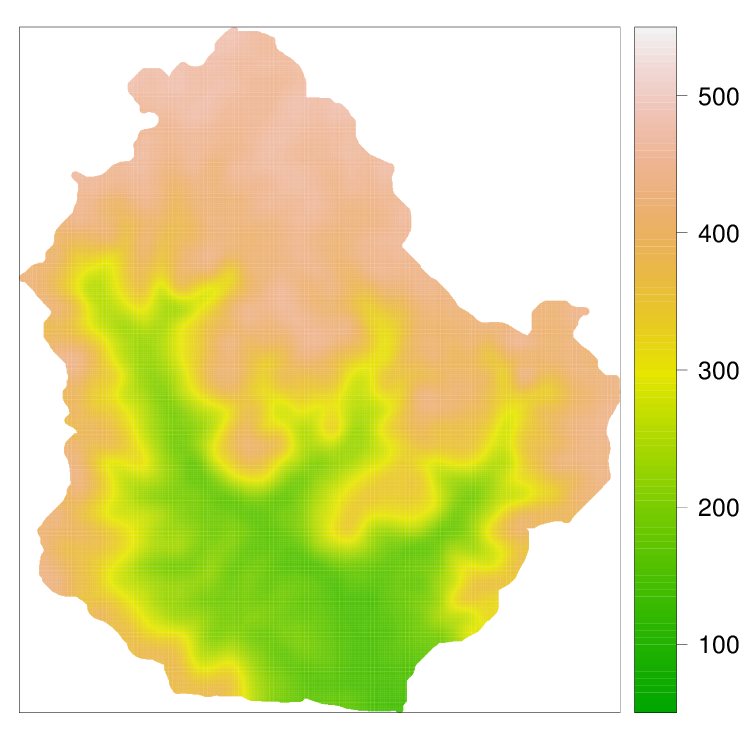
\includegraphics[width=60mm]{chap01FIG4a}
    \end{minipage}
    \begin{minipage}[b]{63mm}
      \subcaption{Spatial resolution: 30~m}
      \label{fig:sat-old}
      \centering
      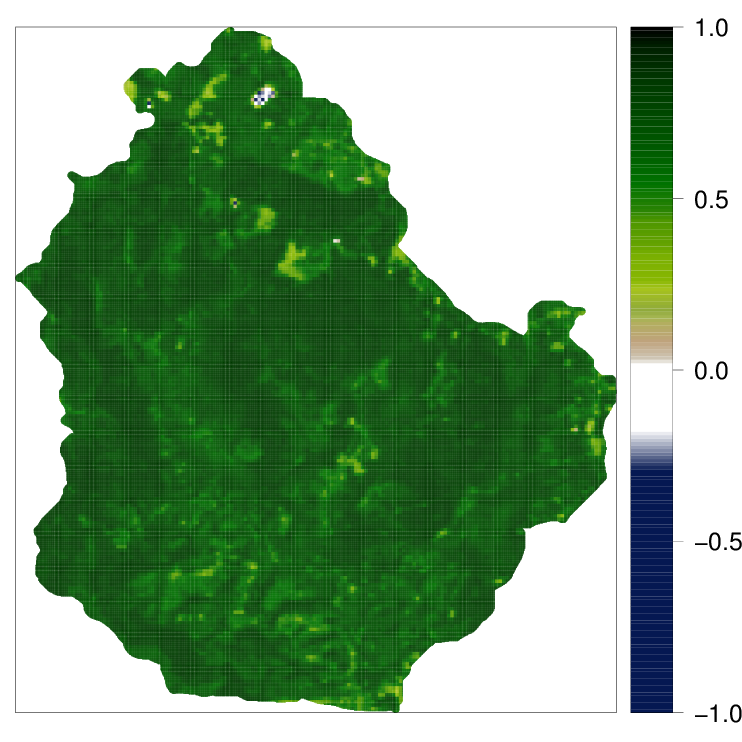
\includegraphics[width=60mm]{chap01FIG4b}
    \end{minipage}
    \begin{minipage}[b]{63mm}
      \subcaption{Vertical spacing of contours: 10~m}
      \label{fig:dem-new}
      \centering
      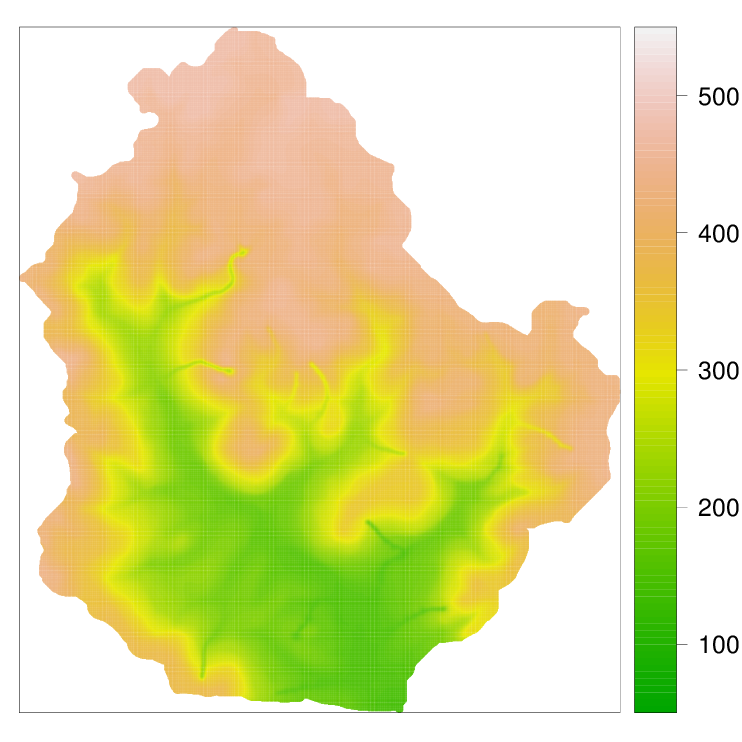
\includegraphics[width=60mm]{chap01FIG4c}
    \end{minipage}
    \begin{minipage}[b]{63mm}
      \subcaption{Spatial resolution: 5~m}
      \label{fig:sat-new}
      \centering
      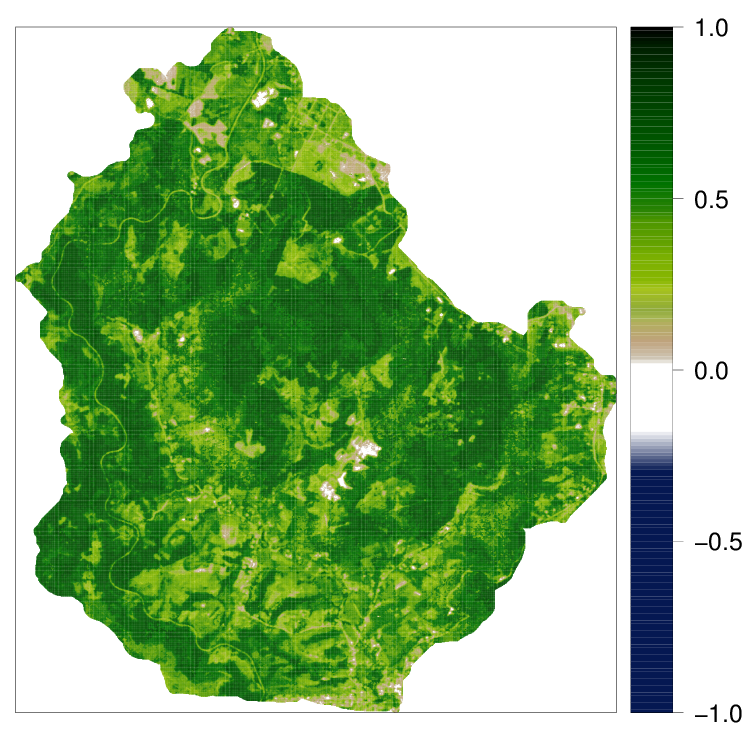
\includegraphics[width=60mm]{chap01FIG4d}
    \end{minipage}
  \caption{Digital elevation models (a, c) and satellite images, depicted using   the normalized difference 
vegetation index (b, d), compared in our study. The less detailed version is displayed at the top, while the 
more detailed version is shown on the bottom.}
  \label{fig:con-covars}
\end{figure}

Eight DEM derivatives were calculated: elevation (\elev), slope (\slp), aspect (\asp), northernness (\nor), 
flow accumulation (\acc), topographic wetness index (\twi), stream power index (\spi), and topographic 
position index (\tpi). \slp{} and \asp{} were calculated using \grass{r.param.scale} with seven window sizes 
(sampling support, analysis scale): 3, 7, 15, 31, 63, 127, and 255. \asp{} was scaled to the standard 
0-360$^\circ$ range and orientation, and was transformed to \nor{} using $\texttt{NOR} = abs(180^\circ - 
\texttt{ASP})$. \twi{} and \spi{} were calculated using \slp{} calculated with different window sizes, and 
\acc{} calculated using \grass{r.watershed}. \tpi{} was calculated using \saga{ta\_morphometry} with the same 
seven window sizes. The combination of DEM derivatives (\elev, \slp, \nor, \twi, \spi, and \tpi) and window 
sizes yielded $p=36$ continuous predictor variables from each DEM.

The less detailed satellite image was acquired by the Landsat-5 Thematic Mapper on December 26, 2010 
(available at Instituto Nacional de Pesquisas Espaciais - Divisão de Geração de Imagens -- 
\href{http://www.dgi.inpe.br/CDSR/}{INPE-DGI}) (\autoref{fig:sat-old}). It has 8~bits radiometric resolution 
and $\sim$~30~m spatial resolution. Spectral bands were orthorectified (Geomatica\textregistered{}
OrthoEngine\textregistered{}) and radiometrically corrected (\grass{i.landsat.toar}). The more detailed 
satellite image comes from the RapidEye constellation (available at Ministério do Meio Ambiente -- 
\href{http://geocatalogo.ibama.gov.br/}{MMA}) (\autoref{fig:sat-new}). It was acquired on November 16, 2012, 
has 16~bits radiometric resolution, 6.5~m spatial resolution, and was orthorectified to 5~m spatial resolution. 
Both images were atmospherically (6S atmospheric model \cite{VermoteEtAl1997}, \grass{i.atcorr}) and 
topographically corrected (\grass{i.topo.corr}). Derived predictor variables are the spectral bands (except 
the thermal band) and vegetation indices (normalized difference vegetation index - NDVI, and soil-adjusted 
vegetation index - SAVI). Eight continuous predictor variables were derived from the Landsat-5~TM image and 
nine from the RapidEye image.

\subsubsection*{Additional processing}
\label{subsubsec:sources-processing}

Soil maps, geologic maps, land use maps, and satellite images were registered with the prediction grid (5-m 
pixel size) using nearest neighbour resampling. \demOld{} was registered using cubic resampling 
\cite{Samuel-RosaEtAl2013c}. Systematic positional errors were corrected using affine transformation 
\cite{Samuel-RosaEtAl2014}.

\subsection{Linear mixed model of spatial variation}
\label{subsec:lmm}

We model each of the soil properties of interest as the outcome of a spatial stochastic process. The model is 
composed of fixed and random effects \cite{HeuvelinkEtAl2001, LarkEtAl2006}. We use the point soil observations 
and spatially exhaustive predictor variables to calibrate the model and predict the outcome of the spatial 
stochastic process at unobserved locations. This fixed effect (deterministic trend), $\mu(\textbf{s})$, 
describes that part of the spatial variation of the soil property that is explained by the covariates. We 
assume here that is a linear function of the predictor variables. The random effect (stochastic residuals, 
latent variables), $\varepsilon(\textbf{s})$, describes that part of the spatial variation that cannot be 
explained by the covariates \cite{Cressie1993}. It is represented by a spatially correlated, Gaussian 
distributed random variable, that is assumed stationary in the mean and covariance. Thus, the linear mixed 
model of spatial variation that we employed is given by

\begin{equation}\label{eq:lmm}
 Z'(\textbf{s}) = \mu(\textbf{s}) + \varepsilon(\textbf{s}) = \sum_{j=0}^{p} 
 \beta_{j}\cdot X_{j}(\textbf{s}) + \varepsilon(\textbf{s}),
\end{equation}

\noindent{where $Z'(\textbf{s})$ is the soil property after Box-Cox transformation, $\mu(\textbf{s})$ and 
$\varepsilon(\textbf{s})$ are defined as above, $\beta_{j}$ are the regression model coefficients, and 
$X_{j}(\textbf{s})$ is the regression model matrix, with $j=0, 1, 2, \ldots, p$, $p$ being the number
of predictor variables. Variable $X_{0}(\textbf{s})$ is taken as unity so that $\beta_{0}$ is the intercept.}

\subsubsection*{Model selection}

We calibrated $m=2^5=32$ multiple linear regression models for each soil property (fitted using ordinary least 
squares, OLS) to model the deterministic trend for each combination of the five covariates (recall from 
\autoref{sec:intro} that each covariate is available at two levels of spatial detail, hence $2^5$ 
combinations). The number of predictor variables used to calibrate each model varied among combinations between 
$p=52$ and $p=62$, because more detailed covariates enabled the derivation of a larger number of predictor 
variables (except the DEM). Backward VIF (variance inflation factor) selection followed by stepwise AIC 
(Akaike's Information Criterion) selection were used to select predictor variables to enter the models 
\cite{Samuel-RosaEtAl2014c, VenablesEtAl2002}.

The $m=32$ multiple linear regression models calibrated for each soil property were ranked using the ratio 
between the regression sum of squares and the total sum of squares. Because stepwise regression results in 
biased models \cite{Harrell2001a}, the ratio of sum of squares was adjusted (${R}^{2}_{adj}$) using the number 
of predictor variables initially offered to enter the model instead of the reduced number of predictor 
variables that entered the model. Next, the five environmental covariates were ranked based on how their level 
of spatial detail related with the calibration of models with improved predictive performance. The relation 
between the level of spatial detail of the covariates and model performance was evaluated using a graphical 
output called model series plot (\Rpackage{pedometrics}, \citeonline{Samuel-RosaEtAl2014c}). Pedological 
evaluation of predictor variables included in the models was omitted because this was beyond our objectives.

The multiple linear regression model calibrated using only the less detailed environmental covariates, which we 
call the \textit{baseline} model, and the multiple linear regression model with the highest ${R}^{2}_{adj}$, 
which we call the \textit{best performing} model, were extended to linear mixed models of 
spatial variation (\autoref{eq:lmm}) for each soil property. Estimation of the parameters of the linear mixed 
models was performed using residual (restricted, marginal) maximum likelihood (REML) \cite{RibeiroEtAl2001, 
LarkEtAl2004}. The spatial correlation function adopted was the exponential function (this is equivalent to the 
Matérn correlation function with smoothness parameter $\nu=0.5$ \cite{Stein1999}).

\subsubsection*{Model validation}
\label{subsec:validation}

Only the \textit{baseline} and \textit{best performing} multiple linear regression and linear mixed models 
calibrated for each soil property were validated. Model validation was performed using leave-one-out 
cross-validation (LOO\-/CV) \cite{BrusEtAl2011}. All model parameters were re-estimated at each LOO\-/CV run 
to reduce bias \cite{LaslettEtAl1987}. LOO\-/CV predicted values were back-transformed from the Box-Cox space 
to the original space of soil properties using stochastic simulation \cite{ChristensenEtAl2001}:

\begin{enumerate}
 \item each predicted value and associated prediction error variance were used to simulate $n = 20,000$ values 
from a Gaussian distribution;
\item simulated values were back-transformed using $Z(s) = (Z'(s) \times \lambda + 1)^{1 / \lambda}$, if 
$\lambda > 0$, and $Z(s) = exp(Z'(s))$, if $\lambda = 0$;
 \item the mean and variance of back-transformed simulated values were used as the predicted value and 
prediction error variance in the original space of soil properties.
\end{enumerate}

Five error statistics were computed from the LOO\-/CV results \cite{JanssenEtAl1995, KempenEtAl2010, 
BrusEtAl2011}. The mean error (\textit{ME}), which measures the prediction bias, the mean absolute error 
(\textit{MAE}) and the root mean squared error (\textit{RMSE}), which measure the prediction accuracy, the 
scaled root mean squared error (\textit{SRMSE}, also known as mean squared deviation ratio), which measures how 
well the prediction error variance matches the squared differences between predicted and observed soil 
property, where $\textit{SRMSE}>1$ indicates under-estimation, while $\textit{SRMSE}<1$ indicates 
over-estimation, and the amount of variance explained (\textit{AVE}, also known as coefficient of determination 
or ratio of scatter), which measures the fraction of the overall spread of observed values that is explained by 
the model. The AVE ranges from 0 to 100, where $\textit{AVE}=100$ is the optimal value.

\subsubsection*{Spatial prediction}
\label{subsec:prediction}

Only the \textit{baseline} and \textit{best performing} linear mixed models calibrated for each soil property 
were used for spatial prediction. Spatial predictions at a fine grid of $\sim$~800,000 point locations were 
made in the Box-Cox space using the best linear unbiased predictor (BLUP) with the empirical estimates of the 
random effects (EBLUP) \cite{LarkEtAl2006}. EBLUP with a fixed effect model is conceptually equivalent to 
kriging with external drift and regression kriging, and mathematically equivalent to kriging with external 
drift and universal kriging. Point predicted values and prediction error variances were back-transformed to the 
original soil property space using stochastic simulation as described above (\autoref{subsec:validation}).

\section{Results}
\label{sec:results}

\subsection{Model series plots}

The model series plot is a graphical description of the relation between the prediction accuracy of multiple 
linear regression models and the environmental covariates used to calibrate them (\autoref{fig:model-series}). 
The magnitude of improvement in prediction accuracy is depicted in the bottom panel by the ${R}^{2}_{adj}$. The 
top panel is interpreted both horizontally and vertically. In the vertical direction we identify which version 
of each covariate was used to calibrate a given model. The less and the more detailed versions are identified 
by the yellow (bright) and green (dark) colours, respectively. The \textit{baseline} model is identified by the 
column containing only yellow cells, while the column with only green cells represents the model calibrated 
using only the more detailed version of each covariate, which we call the \textit{most detailed} model. The 
first important results that we obtain from the model series plots is that a) the \textit{baseline} model is 
not the model with the lowest ${R}^{2}_{adj}$, which we call the \textit{poorest performing} model, and b) the 
\textit{most detailed} model is not the \textit{best performing} model.

\begin{figure}[!ht]
  \centering
    \begin{minipage}[b]{\textwidth}
      \subcaption{}
      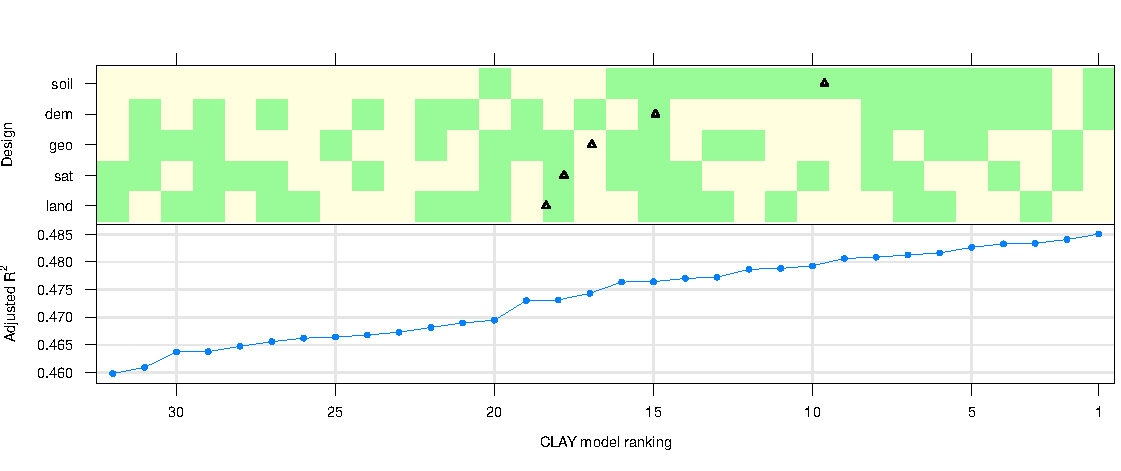
\includegraphics[width=\textwidth]{chap01FIG5a}
    \end{minipage}
    \begin{minipage}[b]{\textwidth}
      \subcaption{}
      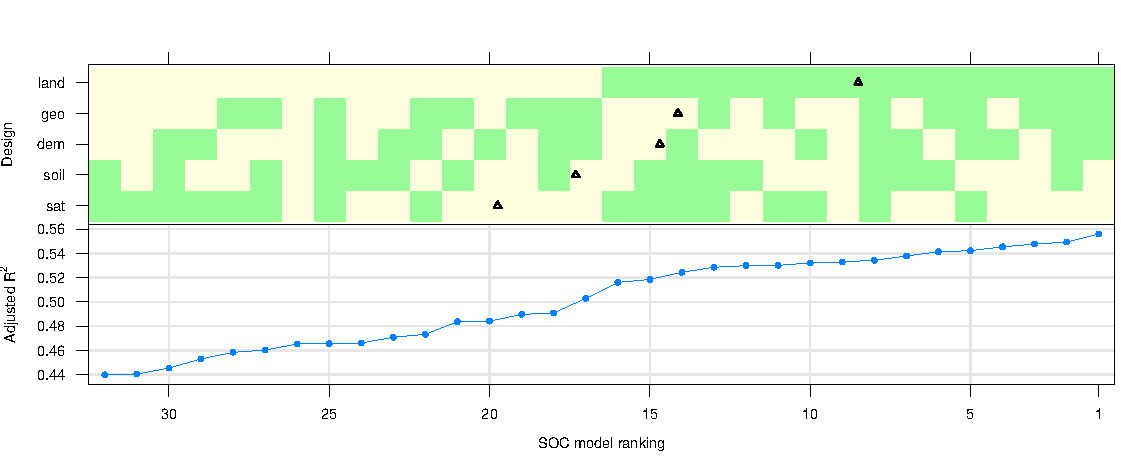
\includegraphics[width=\textwidth]{chap01FIG5b}
    \end{minipage}
    \begin{minipage}[b]{\textwidth}
      \subcaption{}
      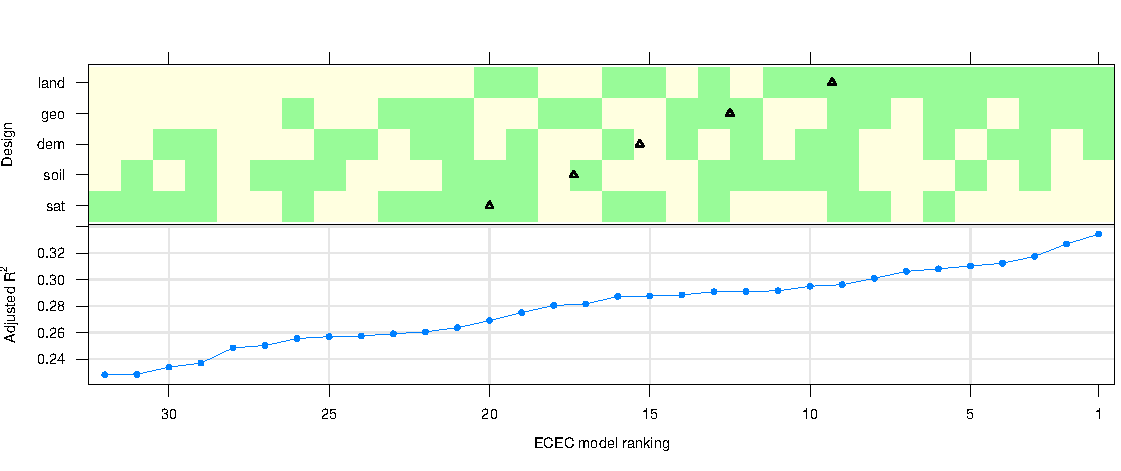
\includegraphics[width=\textwidth]{chap01FIG5c}
    \end{minipage}
  \caption{Model series plots for CLAY (a), SOC (b), and ECEC (c). The less and 
  more detailed version of each environmental covariate are identified by the 
  yellow (bright) and green (dark) colours, respectively. Multiple linear 
  regression models were ranked by their ${R}^{2}_{adj}$. Triangles show the 
  mean ranking of the more detailed covariates (i.e. centre of green cells).}
  \label{fig:model-series}
\end{figure}

The row-wise analysis of the model series plots shows if a model calibrated with the more detailed version of 
a given environmental covariate has a higher prediction accuracy. This information is retrieved by looking at 
the row-wise distribution of green cells -- these cells represent the $m=16$ models calibrated using the more 
detailed version of a given covariate, irrespective of the version of the other covariates. The more 
concentrated the green cells are in the right half of the plot, the larger the relative benefit of using the
more detailed version of that environmental covariate. For example, the top row of the second model series 
plot shows the SOC models calibrated using the two versions of the land use map (\texttt{land}). All green 
cells are on the right half of the plot between rankings 1 and 16 (see the x axis). The four lower rows
show that the green cells of the other four covariates are distributed along the entire ranking range (from 1 
to 32). This means that the relative benefit of calibrating a SOC model with a more detailed land use map is 
larger compared to that of using a more detailed version of the other covariates.

The centre of the row-wise distribution of the green cells for each environmental covariate, calculated as the 
mean ranking, is represented by the triangles. The mean ranking quantifies the relative benefit of using a 
more detailed version of each covariate. For example, the mean ranking of the SOC models calibrated using the 
more detailed land use map is about 8 (top row), while the mean ranking of the models calibrated using the more 
detailed satellite image (\texttt{sat}) is close to 20 (bottom row). Using the more detailed DEM (\texttt{dem}) 
is almost as beneficial as using the more detailed geologic map (\texttt{geo}) -- the mean ranking of the SOC 
models calibrated using the more detailed version of these two covariates is about 15-16 (second and third 
rows). Using the more detailed version of the soil map (\texttt{soil}, fourth row) is not as beneficial as 
using \texttt{land}, \texttt{geo} or \texttt{dem}, but more beneficial than using \texttt{sat}. Because the 
covariates were ranked based on the mean rankings, the covariate displayed in the top row of each model series 
plot is the one which resulted in the largest improvement of the prediction accuracy when the more detailed 
version was used to calibrate the model -- for SOC this is the land use map.

For CLAY, calibrating the models with the more detailed soil map resulted in the largest improvement of the 
prediction accuracy relative to the other environmental covariates. The DEM was the second most beneficial 
covariate (mean ranking of 15), but the benefit of using its more detailed version was similar to that of using 
the more detailed version of any other covariate (mean rankings between 17 and 18). Nine models had a poorer 
prediction performance than the baseline model, ranked 27th, the poorest performing model being that 
calibrated with the more detailed land use map and satellite image. Despite these patterns, calibrating CLAY 
models with the more detailed version of any covariate resulted in a small improvement of the prediction 
accuracy, as evidenced by the small increases of the ${R}^{2}_{adj}$. The difference between the poorest and 
best performing models is less than 3~percentage points (pp). In comparison, for SOC, by simply using the more 
detailed land use map we already obtained a model ranked 9th, an increase of 8~pp in ${R}^{2}_{adj}$ compared 
to the baseline model, ranked 24th.

The same general pattern observed for SOC models was observed for ECEC models -- the more detailed land use map 
results in the largest improvement of the prediction accuracy. The main difference is that calibrating the 
models with the more detailed geologic map was slightly more beneficial for ECEC (mean ranking of 12) than for 
SOC (mean ranking of 14). The poorest performing ECEC model was that calibrated with the more detailed 
satellite image. Using only the more detailed land use map resulted in an improvement of 6~pp in 
${R}^{2}_{adj}$ (model ranked 7th), differing from the best performing model by only 2~pp. Using the more 
detailed version of all environmental covariates except the soil map or satellite image resulted in increases 
of about 6 and 7~pp in ${R}^{2}_{adj}$, respectively. The baseline model was ranked as 28th, which is a higher 
ranking than the models calibrated with all possible combinations of the more detailed satellite image and the 
more detailed soil map and/or DEM.

The patterns observed in the model series plots resulted from the change (increase or decrease) of the 
importance of each environmental covariate on explaining the variance when the more detailed version was used 
(\autoref{tab:drop}). We used the \textit{baseline} and \textit{most detailed} models to quantify this change. 
Each model was refitted dropping one covariate at a time. The difference $\Delta$ between the ${R}^{2}_{adj}$ 
of the model calibrated with all five $q$ covariates (${R}^{2}_{adj}{}_{q=5}$) and the model calibrated without 
the $q$-th covariate ($R^{2}_{adj}{}_{q=5-1}$) was calculated. The more positive $\Delta{R}^{2}_{adj}$ 
becomes, the more beneficial the more detailed version of the $q$-th covariate is for improving prediction 
accuracy. For CLAY, \texttt{dem} and \texttt{land} were the most important covariates in the baseline model, 
while \texttt{geo} was the least important. The importance of \texttt{soil} and \texttt{geo} increased when 
their more detailed version was used (change of $+0.013$~pp for both), while \texttt{sat}, \texttt{land} 
and \texttt{dem} became less important. For SOC and ECEC, \texttt{land} was not the most important covariate in 
the baseline model. But it was the covariate whose importance had the largest positive shift when the more 
detailed version was used ($+0.085$~pp for SOC and $+0.045$~pp for ECEC). \texttt{sat} became less important 
when the more detailed version was used -- see its low ranking in all model series plots. The increase of the 
importance of \texttt{geo} was larger for ECEC ($+0.026$) than for SOC ($+0.013$) -- see the difference in the 
mean ranking of \texttt{geo} in the SOC (14) and ECEC (12) model series plots.

\ctable[
   caption  = {The importance of each environmental covariate$^a$ ($\Delta{R}^{2}_{adj}{}^b$) in the models calibrated with their less and more spatially detailed version.},
   label    = tab:drop,
   pos      = !h,
   %    doinside = \scriptsize\setstretch{1.1}
   doinside = \scriptsize
   ]{lrrcrrcrr}{
   \tnote[a]{Covariate: \texttt{soil} - soil map, \texttt{land} - land use map, \texttt{geo} - geologic map, \texttt{sat} - satellite image, and \texttt{dem} - digital elevation model.}
   \tnote[b]{$\Delta{R}^{2}_{adj} = {R}^{2}_{adj}{}_{q=5} - R^{2}_{adj}{}_{q=5-1}$, where $q$ is the number of covariates included in the model. Negative values result from adjusting the $R^{2}$ using the number of predictor variables initially offered to enter the model instead of the reduced number of predictor variables that entered the model.}
   }{\FL
   \multicolumn{1}{l}{Covariate}&\multicolumn{2}{c}{CLAY}&\multicolumn{1}{c}{}&\multicolumn{2}{c}{SOC}&\multicolumn{1}{c}{}&\multicolumn{2}{c}{ECEC}\NN
   \cline{2-3} \cline{5-6} \cline{8-9}
   \multicolumn{1}{l}{}&\multicolumn{1}{c}{Less}&\multicolumn{1}{c}{More}&\multicolumn{1}{c}{}&\multicolumn{1}{c}{Less}&\multicolumn{1}{c}{More}&\multicolumn{1}{c}{}&\multicolumn{1}{c}{Less}&\multicolumn{1}{c}{More}\ML
   \texttt{soil} &$-0.009$&$ 0.004$&&$-0.006$&$-0.008$&&$ 0.011$&$-0.003$\NN
   \texttt{land} &$ 0.003$&$-0.002$&&$ 0.003$&$ 0.088$&&$-0.004$&$ 0.041$\NN
   \texttt{geo}  &$-0.019$&$-0.006$&&$-0.005$&$ 0.008$&&$ 0.007$&$ 0.033$\NN
   \texttt{sat}  &$-0.010$&$-0.016$&&$ 0.018$&$-0.014$&&$ 0.011$&$-0.029$\NN
   \texttt{dem}  &$ 0.030$&$ 0.001$&&$-0.009$&$ 0.016$&&$-0.035$&$-0.041$\LL
}

\subsection{REML fit of the variogram model}

The small improvement in the prediction accuracy of the CLAY linear mixed model calibrated with the more 
detailed environmental covariates is evidenced by \autoref{fig:lmm}. The shape of the experimental variogram is 
very similar for both baseline and best performing linear mixed models, which is also true for SOC and ECEC. 
However, the sill variance had a very small reduction for CLAY compared to SOC and ECEC. The last two showed a 
more considerable improvement in prediction accuracy. It can also be seen that the number of point observations 
separated by short distances is very small, reducing the accuracy of the estimate of the nugget variance. The 
result is that the estimated nugget variance changes rather erratically from the baseline to the best 
performing models, decreasing for CLAY and SOC, and increasing for ECEC.

\begin{figure}[!ht]
  \begin{center}
    \begin{minipage}[b]{90mm}
      \subcaption{}
      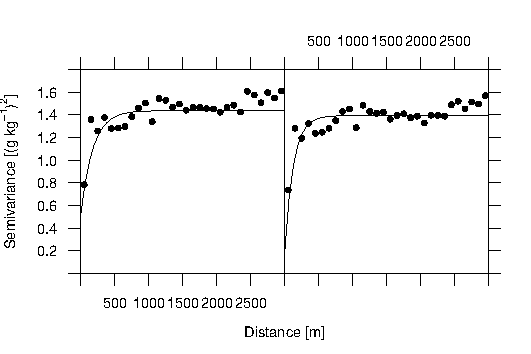
\includegraphics[width=90mm]{chap01FIG6a} 
    \end{minipage}
    \begin{minipage}[b]{90mm}
      \subcaption{}
      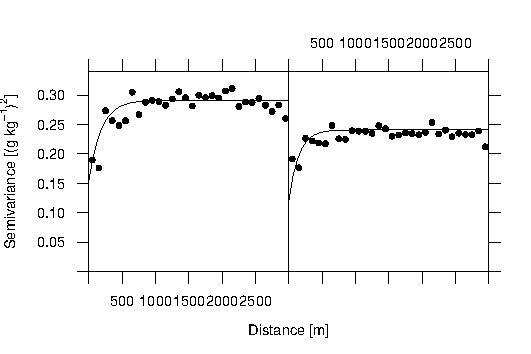
\includegraphics[width=90mm]{chap01FIG6b}
    \end{minipage}
    \begin{minipage}[b]{90mm}
      \subcaption{}
      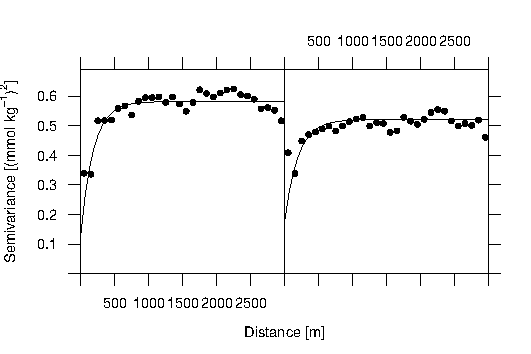
\includegraphics[width=90mm]{chap01FIG6c}
    \end{minipage}
    \caption{Experimental variogram (dots) and REML fit of the linear mixed 
    models (line) for CLAY (a), SOC (b), and ECEC (c). Left -- baseline model.
    Right -- best performing model.}
    \label{fig:lmm}
  \end{center}
\end{figure}

\subsection{Validation}

The LOO\-/CV results indicate that the linear mixed models for CLAY are slightly positively biased, while 
those for SOC and ECEC are slightly negatively biased (\autoref{tab:cv-stats}). For both CLAY and ECEC, the 
\textit{MAE} shows that these models are more accurate than the multiple linear regression models, suggesting 
that the kriging step improves the prediction accuracy.

\ctable[
 caption = [Cross-validation of baseline and best performing models.]{Statistics$^a$ of the LOO\-/CV of 
baseline and best performing multiple linear regression models (LM) and linear mixed models (LMM).},
 label   = tab:chap05-cv-stats,
 notespar,
 pos = !th,
 % doinside = \scriptsize\setstretch{1.1}
 doinside = \small
 ]{llrrrrr}{
 \tnote[a]{Statistics: mean error (\textit{ME}), mean absolute error (\textit{MAE}), root mean squared error 
 (\textit{RMSE}), scaled root mean squared error (\textit{SRMSE}, unitless), and amount of variance explained 
 (\textit{AVE}, percent).}
 }{\FL
   \multicolumn{1}{l}{Model}&\multicolumn{1}{c}{Type}&\multicolumn{1}{c}{\textit{ME}}&\multicolumn{1}{c}{\textit{MAE}}&\multicolumn{1}{c}{\textit{RMSE}}&\multicolumn{1}{c}{\textit{SRMSE}}&\multicolumn{1}{c}{\textit{AVE}}\ML
   \multicolumn{7}{l}{CLAY (g kg$^{-1}$)}\NN
   ~~Baseline&LM&$ 1.31$&$52.1$&$ 72.1$&$0.89$&$56.8$\NN
   ~~&LMM&$ 0.94$&$48.5$&$ 68.8$&$1.03$&$60.7$\NN
   ~~Best performing&LM&$ 1.59$&$51.3$&$ 70.7$&$0.91$&$58.4$\NN
   ~~&LMM&$ 1.08$&$47.8$&$ 68.1$&$1.03$&$61.5$\ML
   \multicolumn{7}{l}{SOC (g kg$^{-1}$)}\NN
   ~~Baseline&LM&$-0.30$&$10.9$&$ 18.9$&$1.22$&$35.8$\NN
   ~~&LMM&$-0.39$&$11.0$&$ 19.4$&$1.43$&$32.5$\NN
   ~~Best performing&LM&$-0.20$&$10.1$&$ 16.9$&$0.91$&$49.0$\NN
   ~~&LMM&$-0.25$&$10.4$&$ 17.6$&$1.16$&$44.3$\ML
   \multicolumn{7}{l}{ECEC (mmol kg$^{-1}$)}\NN
   ~~Baseline&LM&$-0.88$&$70.6$&$112.4$&$0.97$&$22.3$\NN
   ~~&LMM&$-0.32$&$63.3$&$101.1$&$1.32$&$37.1$\NN
   ~~Best performing&LM&$-0.76$&$64.9$&$101.7$&$0.86$&$36.3$\NN
   ~~&LMM&$-0.29$&$62.6$&$ 97.9$&$1.09$&$41.1$\LL
}


Overall, all models had a moderate to poor prediction performance. The errors are, in absolute values, somewhat 
large, mainly for ECEC. The best \textit{AVE} are about 60\% for CLAY, 50\% for SOC and 40\% for ECEC. In 
general, the prediction error variance was under-estimated by the linear mixed models and over-estimated by the 
multiple regression models. The best estimates of the prediction error variance were obtained by both CLAY 
linear mixed models, and the ECEC baseline linear regression model.

For CLAY, the increase in the \textit{AVE} was larger when including a kriging step 
($\Delta\textit{AVE}=3.9$~pp) than when using more detailed environmental covariates 
($\Delta\textit{AVE}=1.6$~pp). In the case of SOC, including a kriging step reduced the \textit{AVE} by 3.2~pp, 
and for ECEC, both strategies increased the \textit{AVE} (\autoref{tab:cv-stats}).

\subsection{Spatial prediction}

Both baseline and best performing linear mixed models captured the same overall pattern of spatial variation of 
the soil properties (\autoref{fig:kriging}). The main difference is that the spatial patterns of the different 
environmental covariates used to calibrate each model produced different features in the prediction maps. For 
example, the CLAY map produced by the best performing model (\autoref{fig:clay-best-pred}) displays abrupt 
changes in the predicted values in the north-northeast due to the use of the more detailed soil map. 
Strongly-marked features following the stream network obtained through the use of the more detailed DEM are 
also observed (Figures \ref{fig:clay-best-pred} and \ref{fig:clay-best-var}).

SOC maps (Figures \ref{fig:soc-best-pred} and \ref{fig:soc-best-var}) show peculiar features in the central 
part of the study area, where predictions reached values as high as \SI{507}{\gram\per\kilo\gram}, while 
the maximum value in the calibration data is \SI{163}{\gram\per\kilo\gram}. The extremely high predicted 
values resulted from the inclusion of the topographic position index derived from the more detailed DEM, using 
a window size of 15~x~15~pixels (\texttt{TPI\_10\_15}) to model the deterministic trend. \texttt{TPI\_10\_15} 
values in the point calibration data range from -7 to 6~m, while in the central part of the study area they 
range from 12 to 31~m. Thus, feature-space extrapolation explains the extremely high predicted values for SOC. 
Abrupt changes in predicted SOC are also observed at locations with low to moderate SOC 
(\SIrange{40}{80}{\gram\per\kilo\gram}). This is caused by using the more detailed land use map.

Predicted ECEC (Figures \ref{fig:ecec-base-pred} and \ref{fig:ecec-best-pred}) had a large dependency on land 
use and geologic maps. Several features observed in the prediction maps derive from these two covariates. The 
influence of land use is seen in the northern part, while in the western, central, and eastern parts the 
influence of both covariates create an irregular pattern in the spatial distribution of ECEC. It is also in 
these parts that the largest prediction error standard deviations occur, following the spatial pattern of the 
covariates.

 \begin{figure}[!ht]
    \centering
    \begin{minipage}[b]{63mm}
      \subcaption{}
      \label{fig:clay-base-pred}
      \centering
      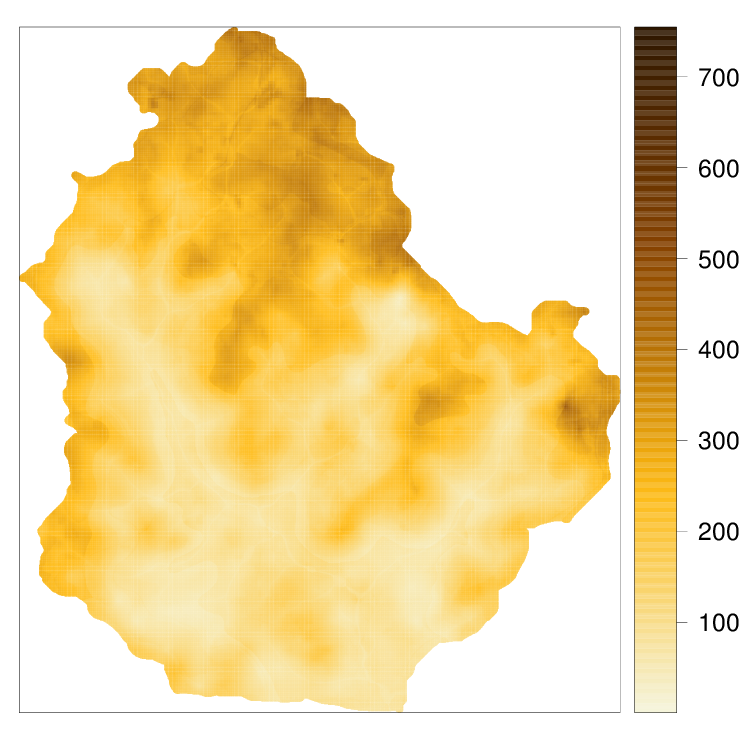
\includegraphics[width=63mm]{chap01FIG7a}
    \end{minipage}
    \begin{minipage}[b]{63mm}
      \subcaption{}
      \label{fig:clay-best-pred}
      \centering
      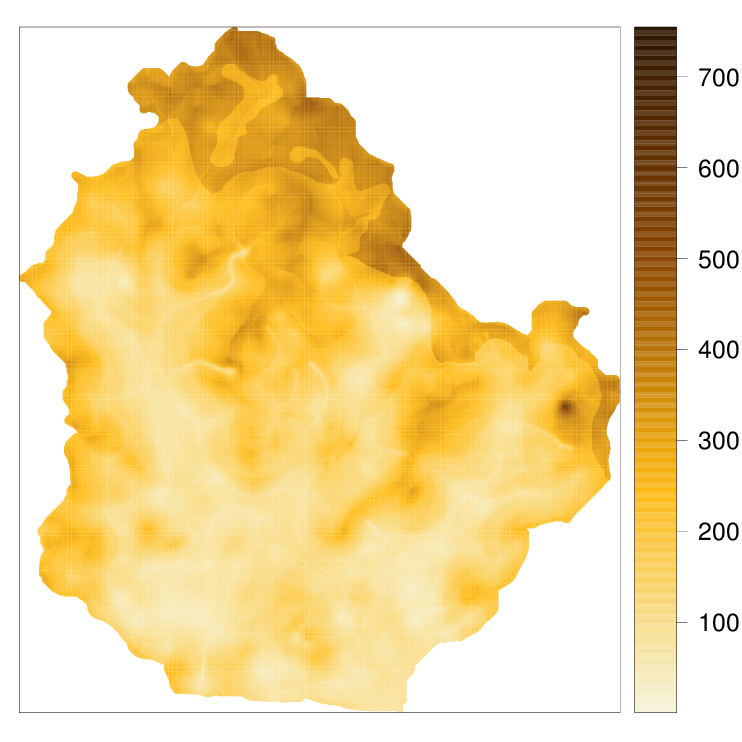
\includegraphics[width=63mm]{chap01FIG7d}
    \end{minipage}
    \begin{minipage}[b]{63mm}
      \subcaption{}
      \label{fig:soc-base-pred}
      \centering
      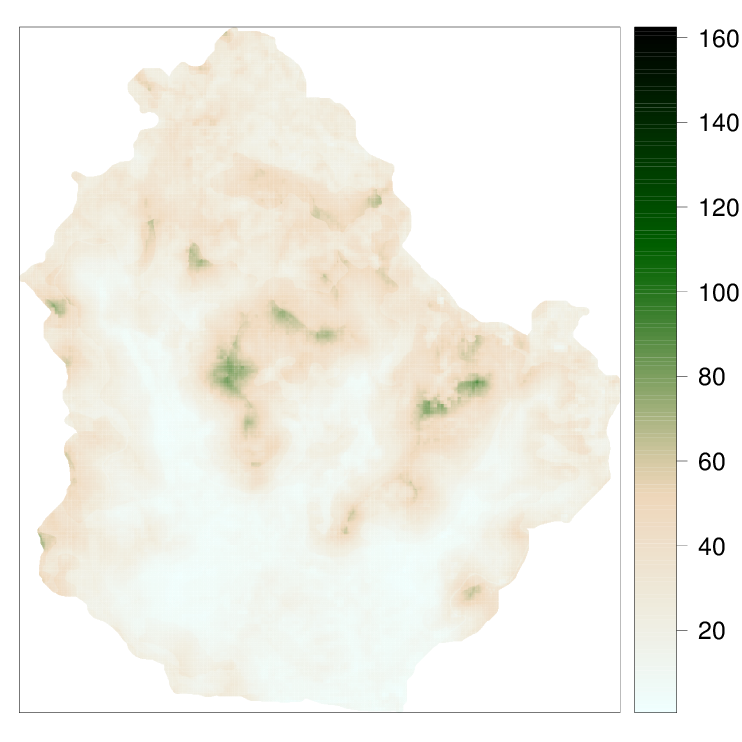
\includegraphics[width=63mm]{chap01FIG7b}
    \end{minipage}
    \begin{minipage}[b]{63mm}
      \subcaption{}
      \label{fig:soc-best-pred}
      \centering
      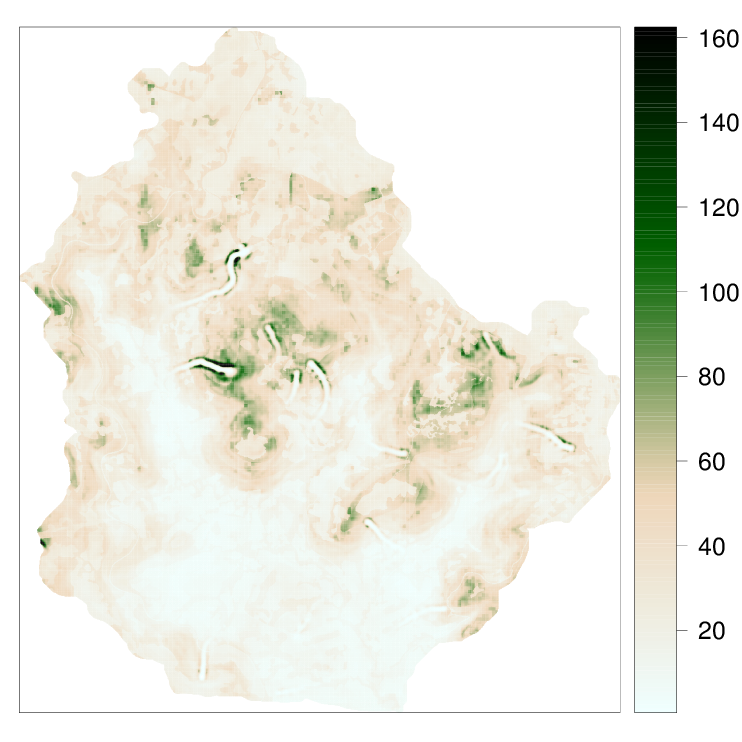
\includegraphics[width=63mm]{chap01FIG7e}
    \end{minipage}
    \begin{minipage}[b]{63mm}
      \subcaption{}
      \label{fig:ecec-base-pred}
      \centering
      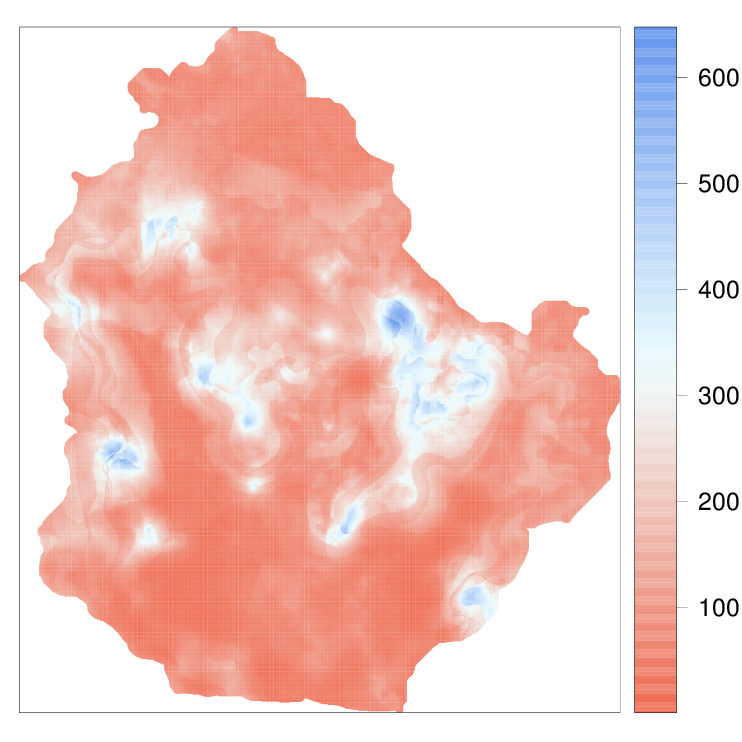
\includegraphics[width=63mm]{chap01FIG7c}
    \end{minipage}
    \begin{minipage}[b]{63mm}
      \subcaption{}
      \label{fig:ecec-best-pred}
      \centering
      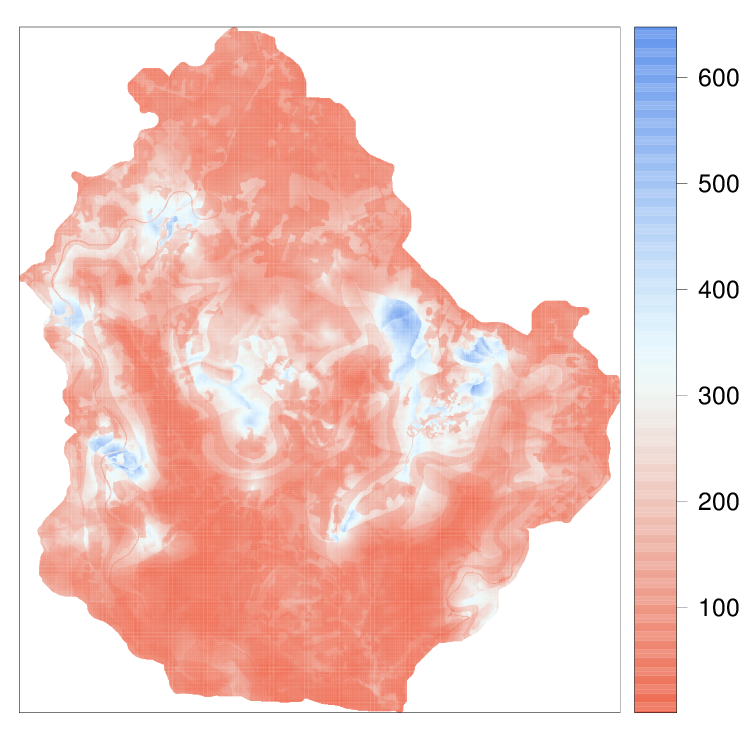
\includegraphics[width=63mm]{chap01FIG7f}
    \end{minipage}
  \caption{Predicted values for CLAY (\si{\gram\per\kilo\gram}) (a, b), SOC (\si{\gram\per\kilo\gram}) (c, d), 
and ECEC (mmol~kg$^{-1}$) (e, f) using the baseline (left) and best performing (right) linear mixed models.}
  \label{fig:kriging}
\end{figure}

\begin{figure}[!ht]
\centering
    \begin{minipage}[b]{63mm}
      \subcaption{}
      \label{fig:clay-base-var}
      \centering
      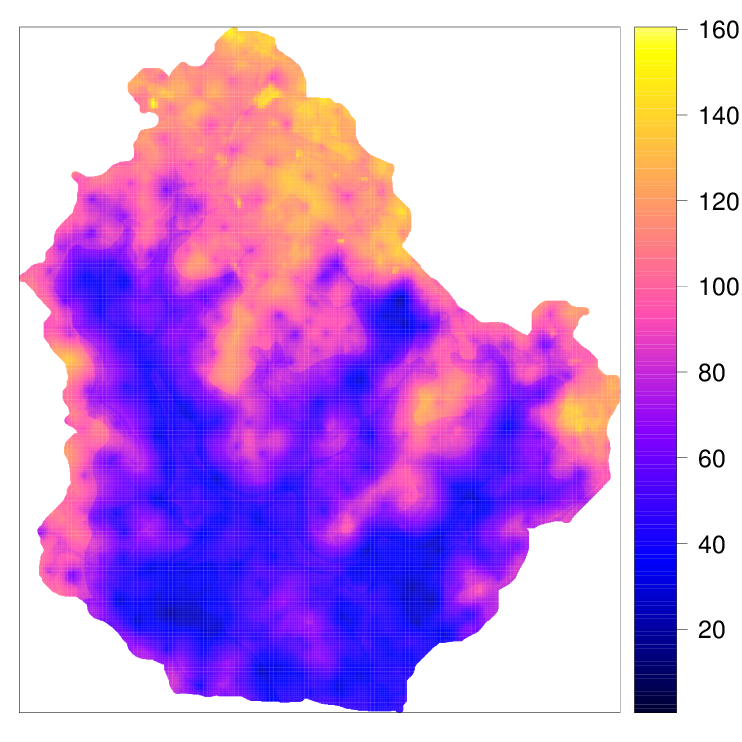
\includegraphics[width=60mm]{chap01FIG8a}
    \end{minipage}
    \begin{minipage}[b]{63mm}
      \subcaption{}
      \label{fig:clay-best-var}
      \centering
      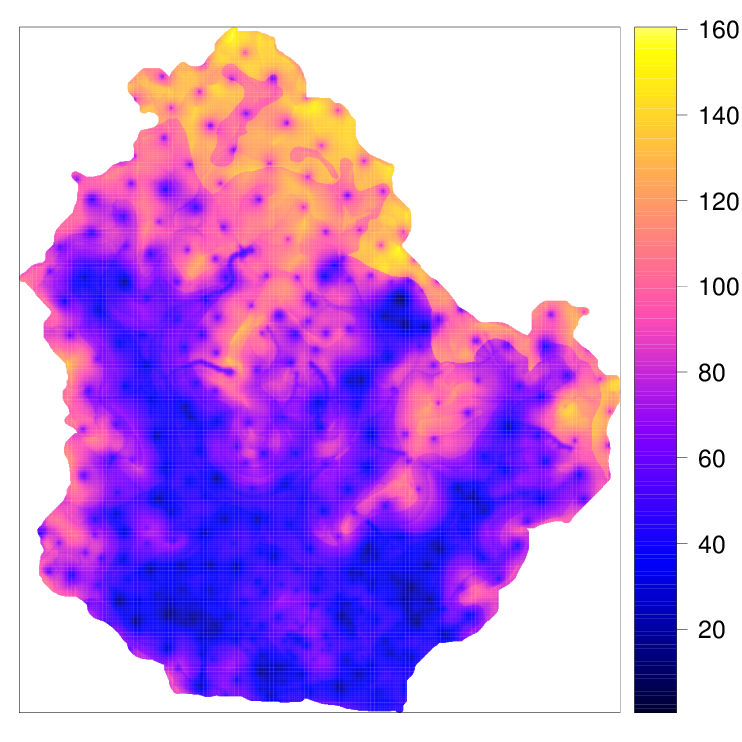
\includegraphics[width=60mm]{chap01FIG8d}
    \end{minipage}
    \begin{minipage}[b]{63mm}
      \subcaption{}
      \label{fig:soc-base-var}
      \centering
      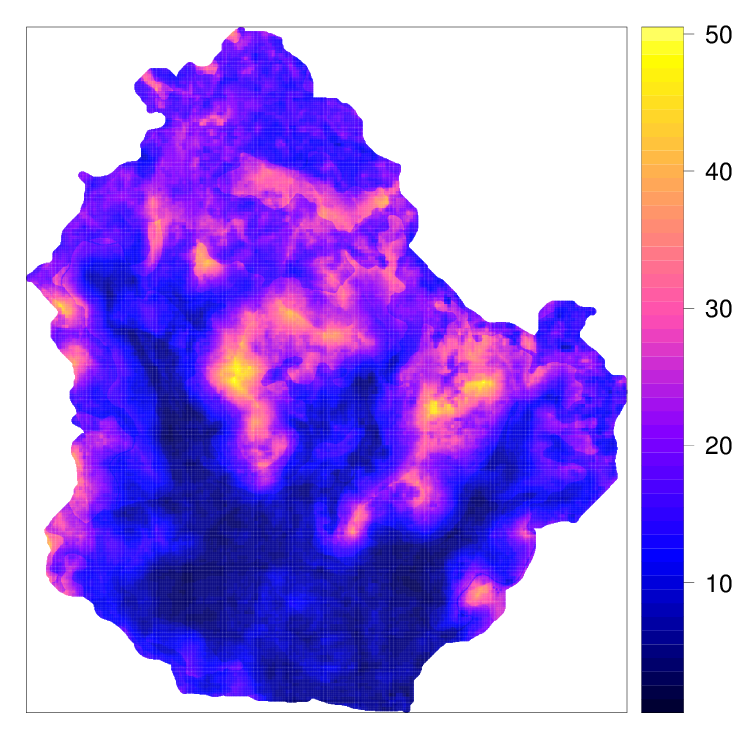
\includegraphics[width=60mm]{chap01FIG8b}
    \end{minipage}
    \begin{minipage}[b]{63mm}
      \subcaption{}
      \label{fig:soc-best-var}
      \centering
      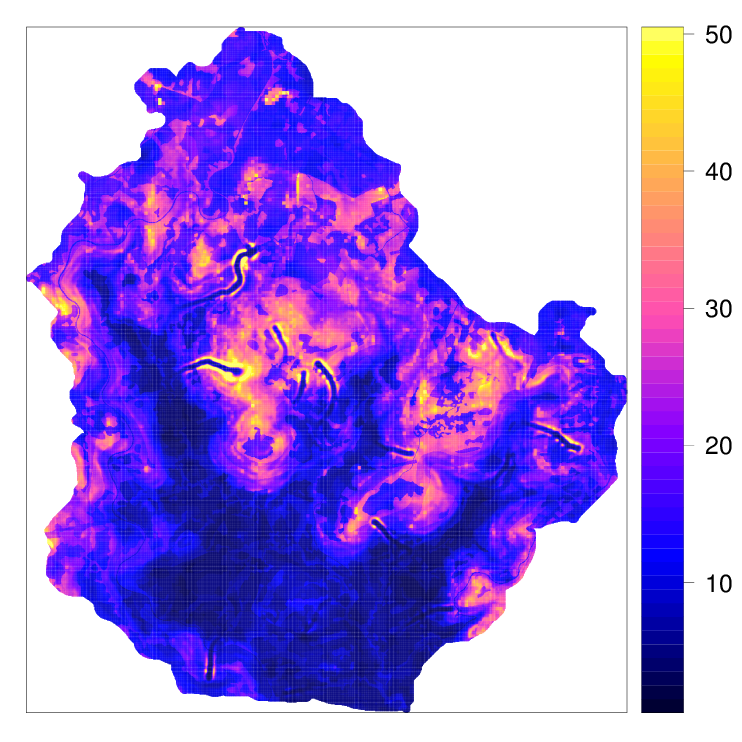
\includegraphics[width=60mm]{chap01FIG8e}
    \end{minipage}
    \begin{minipage}[b]{63mm}
      \subcaption{}
      \label{fig:ecec-base-var}
      \centering
      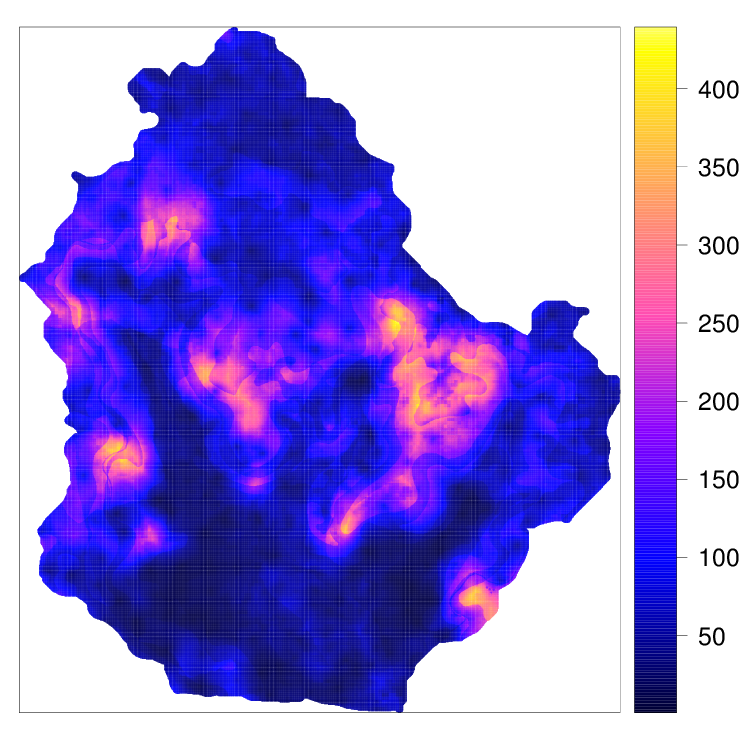
\includegraphics[width=60mm]{chap01FIG8c}
    \end{minipage}
    \begin{minipage}[b]{63mm}
      \subcaption{}
      \label{fig:ecec-best-var}
      \centering
      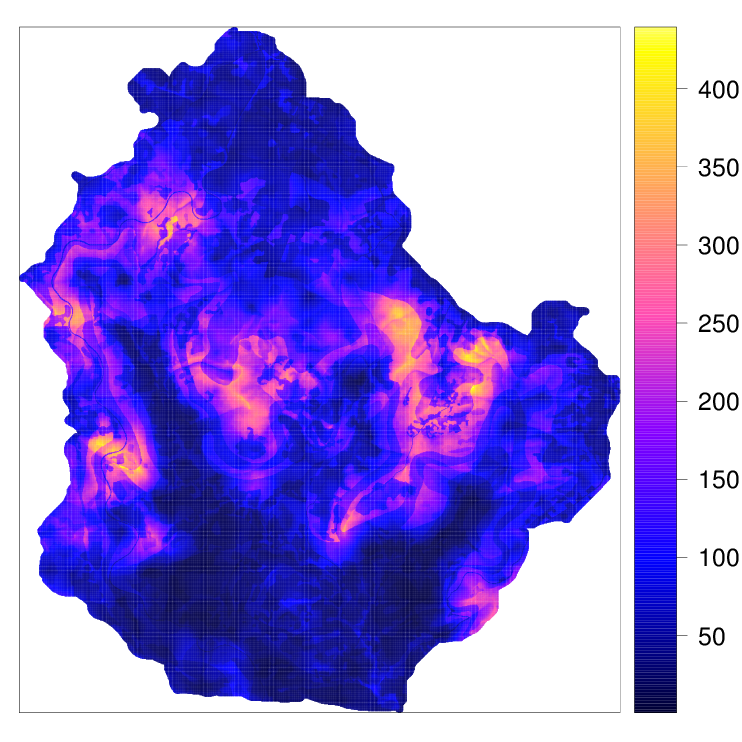
\includegraphics[width=60mm]{chap01FIG8f}
    \end{minipage}
  \caption{Prediction error standard deviations for CLAY (\si{\gram\per\kilo\gram}) (a, b), SOC 
(\si{\gram\per\kilo\gram}) (c, d), and ECEC (mmol~kg$^{-1}$) (e, f) using the baseline (left) and best 
performing (right) linear mixed models.}
  \label{fig:kriging-variance}
\end{figure}

The smallest prediction error standard deviations occur at lower elevations, along the three main streams, and 
close to the water outlet in the southern part of the study area. These areas have the highest density of point 
soil observations used to calibrate the models, and the smallest values for all three soil properties. While 
the first determines the accuracy of the EBLUP, the second influences the final accuracy through the 
back-transformation of predicted values.

\section{Discussion}

Our main goal was to evaluate whether investing in more spatially detailed environmental covariates improves 
the accuracy of soil maps. We saw that calibrating the models with more detailed covariates generally has a 
small to moderate, but positive, impact on the predictions. The magnitude of this benefit depends on the 
magnitude of the increase of the spatial detail of the covariate, on the other covariates included in the 
model, and on the soil property. However, there seems to be a limit above which the increase of spatial
detail has a negative impact on the predictions. In the next two subsections we interpret the results from a 
pedological perspective and assess whether the investment in more detailed covariates is worthwhile or if 
alternatives to improve prediction accuracy should be favoured.

\subsection{Spatio-temporal controls of soil properties}

CLAY was moderately well predicted using less detailed environmental covariates, with small improvement when 
using the more detailed covariates. CLAY was expected to have a strong correlation with topography and parent 
material. This correlation was already considerable when the less detailed DEM and geologic map were used, and 
improved only marginally with the more detailed version. One sensible explanation is that the effective (actual 
rather than theoretical) spatial detail of the two geologic maps was similar, although they had a four-fold 
difference in the size of the minimum legible delineation (see \citeonline{HenglEtAl2006a} for a discussion on 
effective scale). For the DEM, many studies have already suggested that its resolution may be of secondary 
importance when calculating DEM derivatives for digital soil mapping \cite{ZhuEtAl2008, BehrensEtAl2010a, 
MillerEtAl2015}. The influence of land use on CLAY is currently small due to reduction of soil erosion in the 
first decade of the 21st century \cite{MiguelEtAl2012, TenCatenEtAl2012b}. A moderate within-field spatial 
variation may exist due to past erosional processes \cite{MouraBueno2012}, but we lack evidence of how well 
this source of variation was captured in the present-time point soil data.

It is worthwhile to consider the influence of the more detailed soil map on predicting CLAY. Due to its 
production process, the more detailed soil map derives a large amount of spatial detail from the geologic map, 
land use map and DEM -- note that the second-best performing model for CLAY included the more detailed geologic 
map instead of the more detailed soil map (\autoref{fig:model-series}). However, most of the additional spatial 
detail included in the more detailed soil map was probably based on the spatial variation of soil texture, 
because this is a strongly marked soil feature in the area \cite{MiguelEtAl2012}. Soil texture is one of the 
most important soil properties used by soil surveyors in the field to identify mapping units \cite{Legros2006}. 
These findings help explain why in the end the more detailed soil map was the most beneficial for CLAY instead 
of the geologic map.

SOC and ECEC were considerably better predicted when more detailed environmental covariates were used. Our 
expectation that SOC and ECEC would have a strong correlation with land use was confirmed by the fact that this 
covariate explained a large amount of the variance and was highly beneficial for improving the predictions. 
Although the available point soil data are limited to the 2004-2011 period, we believe that land use changes in 
the last 30~years \cite{MiguelEtAl2012, TenCatenEtAl2012b} strongly affected SOC and ECEC. Thus, 
the more detailed land use map is likely to have considerably improved model performance because it is 
up-to-date and, possibly, because it has 40 times more spatial detail than its less detailed version. Despite 
the fact that the two land use maps used in this study were from different time periods, which confounds the 
analysis, the results obtained indicate that a more detailed land use map improves the prediction of SOC. For 
example, the areas used for crop agriculture, which are well know for having lower SOC and ECEC 
\cite{Menezes2008, MouraBueno2012}, are not depicted in the less detailed land use map.

We expected SOC to have a stronger correlation with the DEM than with the geologic map due to its strong 
dependence on erosion, but we observed the contrary. This result my be partially explained by the fact that 
there is a strong relation between geology and topography in the study area \cite{Sartori2009}. Due to its 
production process \cite{MacielFilho1990}, the geologic maps can be interpreted as an aggregated version of a 
DEM. A second sensible explanation is that the effect of erosion on SOC is not that large because erosion was 
considerably reduced in the last decade \cite{MiguelEtAl2012, TenCatenEtAl2012b}. A last possible explanation, 
which integrates the previous two, is the existence of a spatial relation between SOC and CLAY, the last being 
strongly correlated with parent material. These relations help explain why the more detailed DEM was almost as 
beneficial as the more detailed geologic map for SOC predictions. In the case of ECEC, our expectation of a 
strong dependency on a more detailed geologic map for producing more accurate predictions was confirmed.

The observed benefit of the more detailed geologic map and DEM for making more accurate CLAY, SOC and ECEC 
predictions suggests that these soil properties are spatially related in the study area. We also hypothesize 
that the complexity of current land use makes it difficult to achieve SOC and ECEC models with 
performances comparable to CLAY. One important source of variation in forested areas is its use for animal 
grazing \cite{SamuelRosaEtAl2011a}. This influences nutrient cycling and soil nutrient availability 
\cite{SchramaEtAl2013}. Current remote sensing technology is unable to capture the data needed to proxy the 
environmental conditions created by these processes.

\subsection{Using more detailed environmental covariates}

More detailed covariates are usually expected to improve predictions in digital soil mapping 
\cite{CavazziEtAl2013, MaynardEtAl2014}. However, deciding whether to invest or not in more detailed 
covariates requires careful thinking and depends on case-specific elements. We generally saw improvement in 
the predictions in our study, but the improvement was not large and may not outweigh the costs. Also, the 
models calibrated with the more detailed versions of all covariates were not the best performing models. Using 
more detailed satellite images and land use maps degraded CLAY predictions. Although the more detailed
soil map had the largest benefit for CLAY, it may be too costly and impractical since its production usually 
requires having available more detailed versions of all other covariates. For SOC and ECEC, simply using a more 
detailed land use map resulted in considerably more accurate predictions. However, the superior performance may 
not outweigh the extra costs because producing a more detailed land use map usually requires up-to-date field 
observations and satellite images. Thus, the decision to adopt a more detailed covariate for digital soil 
mapping will ultimately depend on a trade-off between the increased accuracy and the extra budget required. It 
may also depend on other potential applications of the covariates, but this is not our concern here.

One interesting observation is that if a less detailed covariate yields poor predictions, its more detailed 
version has the potential to produce larger improvement in model performance. However, this is only a 
potential, not a guarantee. For instance, \citeonline{EldeiryEtAl2008} were not able to increase the $R^2 = 
0.31$ of linear regression models of soil salinity by more than 0.07 points using 7.5 times more detailed 
satellite images. On the other hand, model performance is likely to be hardly improved using more detailed 
covariates if their less detailed version has already produced accurate predictions. This agrees with findings 
by \citeonline{ThompsonEtAl2001} and \citeonline{KimEtAl2014}.

We also observed that the predictions can be degraded when using the more detailed version of covariates. In 
our study, this happened with the satellite image (all three soil properties), land use map (CLAY) and soil map 
(SOC and ECEC). A (small) benefit was observed only when these covariates were used along with the more 
detailed version of other covariates. As pointed out above, such a small benefit may not outweigh the increase 
in mapping costs. The trade-off between reducing model performance and being beneficial seems to depend on how 
much more spatial detail a covariate will have and on its correlation with the soil property. For example, the 
land use map was strongly correlated with SOC and ECEC, but not with CLAY, and its more detailed version 
had 40~times more spatial detail. It helped improve SOC and ECEC predictions, but degraded CLAY predictions, 
resulting in only a small improvement when used along with the more detailed satellite image and geologic map.

If the influence of a more detailed covariate depends on the increase of spatial detail, then the priority 
should be to improve the spatial detail of the most beneficial covariate. This requires solid subject area 
knowledge because empirical evidence from the baseline model may be insufficient. The most beneficial covariate 
is not necessarily that which explained the largest part of the variance in the baseline model (see 
\autoref{tab:drop}). This occurs because increasing the spatial detail reduces the correlation between the 
covariate and the soil property. And also because there is little room to improve a correlation that is already 
high in the baseline model. \citeonline{CavazziEtAl2013} suggest that the more detailed covariate has an 
excess of detail, a ``noise'' that degrades the predictions. This could explain the results for \texttt{sat}: 
higher resolution images can resolve smaller objects (e.g. individual plants) whose spectral behaviours are 
highly variable, adding noise to the \texttt{sat}-soil property correlation; on the other hand, lower 
resolution images capture collections of objects, and thus their variation is smoothed out in the pixel, 
reducing noise.

According to information theory one should optimize (maximize) the correlation between the point soil data and 
the covariates. This was described elsewhere as matching the ``phenomenon scale'' (the spatial pattern of the 
soil property) with the ``analysis scale'' (the spatial pattern of the covariates) \cite{DunganEtAl2002, 
MillerEtAl2014}. Finding the ``optimum'' requires evaluating the strength of the correlation using covariates 
with different levels of spatial detail \cite{DragutEtAl2009, CavazziEtAl2013, MillerEtAl2015}. Our results 
show that this approach may be too costly and impractical. Since digital soil mapping explores only the 
empirical relationship among environmental conditions and soil properties \cite{Grunwald2009}, the ``optimum'' 
is a ``conditional optimum'' -- conditional on the point soil data available. It does not necessarily mean that 
the most accurate predictions will be made, but only that there is a level of spatial detail at which the 
correlation between the covariate and the point soil data is at a maximum. We suggest that instead more 
comprehensive approaches should be used to explore the full potential of the available covariates (see 
\citeonline{BehrensEtAl2010a} and \citeonline{MillerEtAl2015} for examples).

Finally, one must still judge whether the potential improvement in predictions is sufficient given the extra 
costs involved with using more detailed covariates. If the extra budget is spent on deriving more detailed 
covariates, we suggest that it may be better to substantially improve the detail of a less influential
covariate than marginally increase the detail of the most influential covariate. However, other means to spend 
the extra budget should be considered. For instance, it may be more efficient to concentrate on obtaining more 
soil observations. These may focus on better capturing the short range spatial variation \cite{BrusEtAl2007a} 
or improving the representation of the feature space to avoid undesirable extrapolations 
\cite{MinasnyEtAl2006b}.

\section{Conclusions}

This study has shown that:

\begin{enumerate}
 \item Using more detailed environmental covariates results in only a modest increase in the prediction 
accuracy of linear prediction models;
 
 \item A more detailed covariate has a greater potential to improve prediction accuracy when the soil property 
is poorly predicted by its less detailed version;
 
 \item The impact on prediction accuracy when using the more detailed version of a less important covariate 
may depend on which other covariates are included in the model;
 
 \item Choosing whether or not to invest in more detailed covariates depends on the strength of the 
relationship between the covariates and the soil property being modelled, and on the relative difference 
between the less detailed and the more detailed versions of the covariates.
\end{enumerate}

\section*{Acknowledgements}

We are grateful to Dr.~Bradley A.~Miller, from the Leibniz Centre for Agricultural Landscape Research, 
M\"uncheberg, Germany, for his comments during the revision of the manuscript. The following colleagues 
collaborated in different phases of data collection and/or processing: Dr.~Ricardo Simão Diniz Dalmolin, 
Dr.~Edgardo Ramos Medeiros and Jean Michel Moura Bueno (UFSM), Dr.~Pablo Miguel (UFPel), Dr.~Mauro Antonio 
Homem Antunes, Fábio Paes Leme Ferreira, and Anastácia Perci Campos de Almeida (UFRRJ), and Luis Fernando 
Chimelo Ruiz (UFRGS). We are grateful to Dr.~Bas Kempen, Dr.~Tom Hengl, and Marcos Angelini (ISRIC) for their 
helpful comments during the conception of the study and data analysis. We also thank the development teams and 
module/package authors of the many free and open source software (FOSS) and operational system (OS) that were 
used to develop our study. The first author was supported by the CAPES Foundation, Ministry of Education of 
Brazil (Process BEX 11677/13-9). The last author was supported by the CNPq foundation, Ministry of Science and 
Technology of Brazil. The use of the RapidEye images is endorsed by the Corporate Commitment Agreement signed 
between the Federal Rural University of Rio de Janeiro and the Brazilian Ministry of the Environment.

\section*{Note}
This chapter is based on A.~Samuel-Rosa, G.B.M.~Heuvelink, G.M.~Vasques, L.H.C.~Anjos. Do more detailed 
environmental covariates deliver more accurate soil maps? \textit{Geoderma}, v.243--244, p.214--227, 2015.
